\documentclass{cumcmthesis}
\usepackage{url}
\usepackage{array}
\usepackage{tabularx}
\usepackage{longtable}
\usepackage{float}
\usepackage{amsmath}
\numberwithin{equation}{section}
\numberwithin{figure}{section}
\numberwithin{table}{section}

\titlename{基于本地差分隐私的健康手环数据采集与聚合分析系统}
\email{}
\yearinput{2026}
\monthinput{5}
\dayinput{15}

\begin{document}
\maketitle
\newpage
\tableofcontents
\newpage

\begin{cnabstract}

% 摘要内容待补充。

\end{cnabstract}
\cnkeywords{本地差分隐私；健康手环；隐私保护；聚合统计}
\newpage

\section{作品概述}

\subsection{背景分析}

\subsubsection{健康手环数据采集中的三方诉求}

智能手环已经从单一计步设备逐渐发展为睡眠监测、活动分析、异常提醒和长期健康趋势观察的重要入口。平台方希望通过收集用户的睡眠碎片化程度、睡眠时长状态、日均步数分布、站立时长分档等数据，了解群体层面的行为规律，并进一步优化睡眠建议、运动提醒和健康管理算法。

但健康手环数据天然处在“有统计价值”和“有隐私风险”的交叉位置。平台真正需要的是群体统计结果，例如“高碎片化睡眠用户占比”“不同步数区间用户分布”“夜间异常提醒触发比例”等，而不是单个用户的真实原始记录或健康诊断结论。用户担心的也不仅是平台直接收集疾病、BMI、心理健康风险等敏感信息，更担心平台或攻击者通过看似普通的行为摘要反推出个人敏感状态。

因此，本作品面对的核心矛盾可以概括为：平台需要收集可用于统计分析的非敏感属性，用户希望避免由这些属性间接暴露个人敏感状态，监管和社会则要求数据采集过程具备可解释、可控制、可落地的隐私保护机制。作品的目标并不是阻断所有数据流动，而是在“原始数据不出端”的前提下，使平台仍能获得可用的群体统计结果，同时降低用户个体隐私被推断的风险。

\subsubsection{从直接隐私泄露到间接隐私泄露}

传统隐私保护问题通常关注“直接隐私泄露”。例如，平台如果直接询问用户是否属于高 BMI 类别、是否存在代谢风险、是否处于心理健康高风险状态，那么被采集字段本身就是敏感属性 S。此时，标准本地差分隐私（Local Differential Privacy，LDP）的基本做法是让用户在本地对敏感属性 S 进行随机扰动，平台只接收扰动后的结果。

本作品关注的是更贴近健康手环实际应用的“间接隐私泄露”。在本系统中，平台并不直接采集心理健康风险、代谢风险或 BMI 类别等敏感属性 S，而是采集睡眠碎片化等级、睡眠时长状态、步数分桶等非敏感属性 A。单独看，A 只是行为摘要或设备监测结果；但如果 A 与 S 存在统计相关性，平台后台或攻击者就可能利用已有经验、公开数据或系统样本中的条件分布关系，从 A 反推出 S 的可能取值。

以本作品选定的主例子为例：平台希望统计用户的“睡眠碎片化等级 A”，用于判断群体睡眠稳定性和优化睡眠提醒。睡眠碎片化等级本身不是诊断结论，也不是平台明确索取的敏感信息；但若历史数据或研究经验表明“高碎片化睡眠”与“心理健康风险 S”存在统计相关性，那么用户原样上传 A 后，攻击者就可能根据 A 推断用户是否属于较高心理健康风险群体。由此可见，本作品要解决的不是“平台直接采集 S”的问题，而是“平台采集 A 时，A 可能成为推断 S 的线索”的问题。

\subsubsection{本系统中的属性设定与风险关系}

为了使报告、系统和实验保持统一，本文将健康手环场景中的属性关系分为两类：第一类是间接隐私泄露场景，即平台采集的字段本身为非敏感属性 A，但它与敏感属性 S 相关；第二类是混合隐私风险场景，即同一个字段中既包含直接敏感取值，也包含本身不敏感但可能与其他敏感属性相关的取值。

在报告主线中，建议将“睡眠碎片化等级 A 与心理健康风险 S”作为贯穿性主例子，用于解释问题动机、条件分布、内在不确定性和参数重校准；将“睡眠时长状态”“步数分桶”“站立时长分档”等作为协议适配的补充例子；将“夜间异常状况字段”作为混合隐私风险的独立例子，避免把间接泄露和混合泄露混在同一组属性里。

\begin{table}[htbp]
\centering
\small
\begin{tabularx}{\textwidth}{|>{\raggedright\arraybackslash}X|>{\raggedright\arraybackslash}X|>{\raggedright\arraybackslash}X|>{\raggedright\arraybackslash}X|>{\raggedright\arraybackslash}X|}
\hline
场景类型 & 采集字段 & 字段性质 & 保护目标 & 在系统中的作用 \\ \hline
主线例子 & 睡眠碎片化等级 & 非敏感属性 A & 心理健康风险 S & 贯穿问题引入、条件分布、参数重校准和创新点一 \\ \hline
补充例子 & 睡眠时长状态 & 非敏感属性 A & 心理健康风险 S & 用于说明相关性较弱时可以减少不必要噪声 \\ \hline
补充例子 & 日均步数分桶 & 高基数非敏感属性 A & BMI/代谢风险 S & 用于说明高基数字段下的协议适配 \\ \hline
补充例子 & 日均站立时长分档 & 多值非敏感属性 A & BMI 类别 S & 用于说明多值分档场景 \\ \hline
混合例子 & 夜间异常状况字段 & 敏感取值与非敏感相关取值并存 & 低血氧、心率异常等直接敏感取值，以及年龄段等潜在敏感属性 & 用于解释两阶段扰动 TSP \\ \hline
\end{tabularx}
\end{table}

\subsubsection{传统本地差分隐私方案的困境}

本地差分隐私是一类适用于不可信聚合方场景的隐私保护技术。其基本思想是：用户不直接上传真实值，而是在本地设备上先通过随机机制进行扰动，再将扰动后的结果发送给平台。这样，即使平台后台不完全可信，也难以从单个上报值中确定用户真实输入。

对任意两个可能输入 v₁、v₂ 以及任意输出集合 O，若随机机制 M 满足 Pr[M(v₁)∈O] ≤ e\textasciicircum{}ε·Pr[M(v₂)∈O]，则称该机制满足 ε-本地差分隐私。其中，ε 是隐私预算，ε 越小，隐私保护越强，扰动通常也越大。在随机响应类协议中，p 通常表示真实值被如实上报的概率，q 表示真实值被扰动为其他取值的概率。

如果把健康手环中所有与敏感属性相关的非敏感属性 A 都简单地“当作完全敏感属性”处理，那么传统 LDP 可以提供保守的保护思路，但会带来明显效用损失。原因在于，传统参数设计通常主要依赖 ε 和属性域大小 d，而不显式区分 A 与 S 的实际相关性强弱。例如，睡眠时长状态与心理健康风险之间可能只有弱相关，攻击者本来就难以通过该字段推断 S；若仍按最坏情况强行加噪，会使平台获得的群体统计结果严重失真。

因此，传统方案的不足不在于 LDP 本身失效，而在于它没有充分利用健康手环数据中已经存在的“相关性不确定性”。本作品希望在不弱化隐私目标的前提下，把 A 与 S 之间的条件分布纳入参数计算：当 A 对 S 的区分能力较弱时，减少不必要噪声；当 A 对 S 的区分能力较强时，保持足够扰动强度。这样既回应用户对隐私的担忧，也尽量保留平台统计分析所需的数据价值。

\subsection{相关工作与不足}

\subsubsection{本地差分隐私与经典扰动协议}

本地差分隐私已经成为本地数据采集场景中的重要隐私保护框架。常见协议包括随机响应（Randomized Response，RR）、广义随机响应（Generalized Randomized Response，GRR）和一元编码（Unary Encoding，UE/OUE）等。RR 适合二值属性，GRR 适合有限多值属性，OUE 更适合取值空间较大、分布较稀疏的属性。

对应到本项目系统，RR 可用于“是否触发睡眠异常提醒”等二值事件；GRR 可用于“睡眠时长状态”“站立时长分档”等多值离散属性；OUE 可用于“每日步数分桶”等取值较多的高基数属性。上述协议为系统实现提供了基础组件，但其默认参数并不考虑健康手环属性与敏感状态之间的具体相关性，因此仍需要在项目场景中进行再设计。

\subsubsection{面向间接推断风险的现有不足}

在直接隐私泄露场景中，平台采集的字段本身就是敏感属性，因此对该字段做 LDP 扰动是自然选择。但在本作品关注的间接泄露场景中，平台采集的是非敏感属性 A，保护目标却是未被直接采集的敏感属性 S。此时，隐私风险来自 A 与 S 之间的统计相关性，而不是 A 本身的敏感性。

现有方案通常存在四方面不足：第一，扰动强度缺乏相关性感知，难以区分高风险属性和低风险属性；第二，未充分利用 A 与 S 之间天然存在的不确定性，导致对低风险字段过度加噪；第三，对同一字段内不同取值诱发不同泄露模式的混合场景缺少系统化处理；第四，许多研究集中在理论协议层面，缺少与具体产品系统结合的端云协同实现路径。

这些不足决定了本作品不能只把专利或论文中的抽象流程照搬到报告中，而需要围绕健康手环系统重新组织表达：先明确系统收集哪些属性、保护哪些属性，再说明如何估计条件分布、如何选择内在不确定性参数、如何在用户端完成本地扰动，以及服务端如何完成聚合校正。

\subsection{作品特色}

\subsubsection{以健康手环为载体的场景化隐私建模}

本作品以健康手环隐私保护系统为载体，将抽象的“相关非敏感属性采集”问题转化为更具体的健康数据采集问题。系统不直接收集用户的心理健康风险、代谢风险或 BMI 类别等敏感状态，而是围绕平台确有统计需求的睡眠、活动和异常提醒数据进行保护设计。

这种场景化建模的好处在于：一方面，平台仍然能够获得用于算法优化的群体统计结果；另一方面，报告中的每一个技术符号都有实际含义，A 不再只是抽象变量，而是睡眠碎片化等级、睡眠时长状态或步数分桶；S 也不再只是公式中的敏感属性，而是用户不希望被平台或攻击者推断出的健康风险状态。

\subsubsection{内在不确定性驱动的按需加噪}

本作品将“内在不确定性”作为连接场景和算法的核心概念。直观地说，如果不同敏感状态 S 下某个非敏感属性 A 的分布差异很小，那么攻击者即使知道 A，也很难判断用户属于哪一种 S；此时 A 本身已经带有较强的不确定性，系统可以减少额外扰动。反之，如果某个 A 在不同 S 下差异明显，说明 A 对 S 的区分能力较强，系统就需要施加更强扰动。

例如，在睡眠时长状态与心理健康风险的关系较弱时，不同风险群体中“睡眠时长合理”的出现概率可能比较接近，攻击者难以仅凭该字段判断用户风险；而睡眠碎片化等级若与心理健康风险差异更明显，就需要更强的扰动保护。系统通过条件分布 Pr(A|S) 计算内在不确定性参数，并据此重新标定 p、q，使噪声强度尽量贴合实际推断风险。

\subsubsection{四类健康手环数据的差异化协议适配}

健康手环采集的数据形态并不单一：有二值事件、多值分档、高基数分桶，也有敏感取值和非敏感相关取值混合在同一字段中的复杂情况。为了避免“一个协议套所有字段”造成保护不足或效用损失，本作品将不同数据形态分别映射到适合的扰动协议。

\begin{table}[htbp]
\centering
\small
\begin{tabularx}{\textwidth}{|>{\raggedright\arraybackslash}X|>{\raggedright\arraybackslash}X|>{\raggedright\arraybackslash}X|>{\raggedright\arraybackslash}X|>{\raggedright\arraybackslash}X|}
\hline
协议简称 & 协议定位 & 适用数据形态 & 本项目对应字段 & 设计重点 \\ \hline
ARR & 自适应随机响应 & 二值事件 & 是否触发睡眠异常提醒 & 根据 A 与 S 的相关性调整二值扰动概率 \\ \hline
AGRR & 自适应广义随机响应 & 多值分档 & 睡眠时长状态、站立时长分档 & 在多值属性上结合 α、β 重校准 p、q \\ \hline
AOUE & 自适应优化一元编码 & 高基数稀疏属性 & 每日步数分桶 & 降低高基数场景下传统 GRR 误差过大的问题 \\ \hline
TSP & 两阶段扰动 & 混合隐私风险字段 & 夜间异常状况字段 & 先对齐不同泄露模式，再进行统一扰动 \\ \hline
\end{tabularx}
\end{table}

\subsubsection{端云协同的轻量化系统架构}

本作品不仅关注扰动协议本身，还设计了适配健康手环设备能力的系统实现路径。服务端负责完成相对复杂的条件分布建模、内在不确定性参数选择、扰动参数计算和聚合校正；用户端或本地 APP 只接收必要参数，并对本地真实属性执行轻量级随机扰动。

在该架构下，原始数据不离开用户端，平台接收的是扰动后的 Ã；服务端通过无偏估计或校正公式恢复群体统计分布。复杂计算集中在服务端，用户端操作保持简单，既降低了手环侧计算和通信负担，也便于后续在不同健康数据字段之间扩展。

\subsection{应用前景分析}

本项目虽然以健康手环为主要落地场景，但其方法并不局限于单一产品形态。只要一个场景满足“平台需要收集 A、A 本身不是直接敏感属性、A 与用户敏感属性 S 存在统计相关性、平台关注群体统计而非个体真实值”这四个条件，就可以考虑采用类似的内在不确定性驱动扰动机制。

\begin{table}[htbp]
\centering
\small
\begin{tabularx}{\textwidth}{|>{\raggedright\arraybackslash}X|>{\raggedright\arraybackslash}X|>{\raggedright\arraybackslash}X|>{\raggedright\arraybackslash}X|}
\hline
扩展领域 & 平台需要的 A & 可能泄露的 S & 为什么适用本方法 \\ \hline
智能家居 & 设备启停摘要、用电模式、夜间活动频次 & 独居状态、家庭作息、脆弱人群状态 & A 本身是设备行为摘要，但可推断家庭敏感状态 \\ \hline
电商 App & 浏览节律、加购时段、品类偏好 & 孕期状态、育儿阶段、经济压力 & 平台需要群体营销统计，但单个用户画像应被保护 \\ \hline
车联网 & 充电时段、停车时长、路线摘要 & 居住区域、工作地点、出行规律 & 交通行为数据与位置敏感信息存在相关性 \\ \hline
校园/企业健康服务 & 运动打卡频次、睡眠建议响应情况 & 健康风险、心理压力、作息异常 & 适合做群体健康趋势统计，但不应暴露个体状态 \\ \hline
\end{tabularx}
\end{table}

因此，本作品的价值不仅在于完成一个健康手环隐私保护原型，更在于提供一种可迁移的设计思路：先识别非敏感采集属性 A 与敏感保护属性 S 的关系，再利用条件分布度量内在不确定性，最后根据具体数据类型选择合适的本地扰动和聚合方案。

\section{作品设计与实现}

\subsection{作品系统总体架构}

\subsubsection{设计目标}

针对传统本地差分隐私（LDP）机制在收集与非敏感属性统计相关的属性时存在过度扰动、效用低下的问题，本作品设计并实现了一个基于内在不确定性的本地差分隐私演示系统。系统以健康手环数据采集为应用场景，主要实现的目标包括：

隐私保护——通过ARR、AGRR、AOUE、TSP四种协议，对不同类型属性提供隐私保障

效用优化——利用内在不确定性()动态校准扰动参数，降低噪声、提升收集方的数据可用性

完整闭环——覆盖属性配置→策略下发→用户端采集→本地扰动→服务端聚合估计的全流程

可视化演示——直观展示扰动前后分布对比、MSE、一致性等评估指标

\subsubsection{作品实现的核心功能}

本作品以健康手环数据采集为应用场景，在用户端收集用户是否触发睡眠异常提醒、日均站立时长、每日步数、睡眠质量评分等非敏感属性，计算其与年龄段、BMI等敏感属性的内在不确定性，利用ARR等协议对参数进行扰动，并在管理端对数据进行聚合攻击，分析比较聚合估计的效用并进行可视化演示交互。整个实现流程图如下。

\begin{figure}[htbp]
\centering
\includegraphics[width=0.8\textwidth]{2-1.png}
\end{figure}
实现的核心功能包括：四种隐私保护协议的自适应扰动、内在不确定性参数的自动计算、扰动参数的动态重校准、服务端聚合估计与效用评估、可视化演示与交互等。

系统针对四个非敏感属性，实现了四种隐私保护协议的自适应扰动。

\begin{table}[htbp]
\centering
\small
\begin{tabularx}{\textwidth}{|>{\raggedright\arraybackslash}X|>{\raggedright\arraybackslash}X|>{\raggedright\arraybackslash}X|}
\hline
非敏感属性 & 对应敏感属性 & 使用协议 \\ \hline
是否触发睡眠异常提醒 & 年龄 & ARR \\ \hline
日均站立时长 & BMI & AGRR \\ \hline
每日步数 & BMI & AOUE \\ \hline
睡眠质量评分 & 年龄 & TSP \\ \hline
\end{tabularx}
\end{table}

系统实现了内在不确定参数的自动计算。利用公开数据集，计算敏感属性S与非敏感属性A的条件概率分布，并根据对应规则选定内在不确定性参数。

根据ARR、AGRR、AOUE、TSP四种协议，对扰动参数动态重校准，计算出最优扰动参数。

服务器收集所有用户的扰动数据后，执行无偏估计还原真实统计分布，并计算效用评估指标，如均方误差（MSE）、平均绝对误差（MAE）、一致性等。

实现可视化演示与交互。在用户端可以选择任务，执行本地扰动并上传扰动后的数据；在管理端可以配置属性变量设置ε值并发布任务，收集上传数据整合。同时，可以模拟多组数据的上报并进行集合，展示聚合结果与实际结果对比表以及MSE/MAE 等指标。

\subsubsection{系统架构}

作品整个系统架构大致分为四层，包括页面展示层，业务逻辑层，核心算法层、数据存储层。

\begin{figure}[htbp]
\centering
\includegraphics[width=0.8\textwidth]{2-2.png}
\end{figure}

页面展示层主要实现前端页面的展示，技术栈主要为Vue 3 + Element Plus + ECharts，包括首页（Home.vue）、登录页（Login.vue）、注册页（Register.vue）的页面设计；以及在用户端中主页面（UserDevice.vue）、四个协议的结果展示及动画（AgrrMultiClientUploadDemo.vue 等），模拟演示聚合结果；管理端中仪表盘（Dashboard.vue），配置属性（AttrConfig.vue），数据集列表（DatasetList.vue），聚合结果（AggregateResult.vue），场景说明（ScenarioOverview.vue），误差评估（ArrExperimentComparison.vue）等。此外，由路由负责实现页面导航、权限控制、角色隔离等功能。

业务逻辑层实现状态管理以及状态流转。在系统中存储当前状态文件，包括用户认证与信息管理，任务生命周期管理，属性配置管理等。通过存储的当前状态，实现在各个页面之间的状态流转，如传递任务，上报数据等。存储文件信息如下表所示。

\begin{table}[htbp]
\centering
\small
\begin{tabularx}{\textwidth}{|>{\raggedright\arraybackslash}X|>{\raggedright\arraybackslash}X|>{\raggedright\arraybackslash}X|}
\hline
存储文件 & 存储内容 & 核心状态 \\ \hline
user.js & 用户认证与信息管理 & 用户密码等 \\ \hline
task.js & 任务生命周期管理 & 当前任务 \\ \hline
attributeConfig.js & 属性配置管理 & 配置属性 \\ \hline
\end{tabularx}
\end{table}

核心算法层实现LDP的核心算法，包括各个协议的参数计算（ldpAlgorithms.js），数据处理工具（dataProcessing.js），敏感属性数据生成（saGenerator.js）、聚合计算（aggregateMetrics.js）以及TSP协议专用实现（tspProtocol.js ）等。

数据存储层主要实现存储数据，包括用户上报数据以及条件概率数据集等。

\subsection{核心技术实现}

\subsubsection{数据库存储实现}

本系统为前端演示型项目，核心目标是展示基于内在不确定性的本地差分隐私算法效果，而非大规模数据存储。综合考虑部署便捷性和演示流畅度，系统采用浏览器本地存储（localStorage）作为数据持久化方案，无需配置后端数据库服务器。所有用户数据、任务配置、聚合结果均存储在用户浏览器的 localStorage 中，通过 JavaScript API 进行读写操作。系统共设计 5 个核心存储对象，分别管理用户、任务、属性配置、提交数据等，如下表所示。

\begin{table}[htbp]
\centering
\small
\begin{tabularx}{\textwidth}{|>{\raggedright\arraybackslash}X|>{\raggedright\arraybackslash}X|>{\raggedright\arraybackslash}X|>{\raggedright\arraybackslash}X|}
\hline
存储 Key & 存储内容 & 数据类型 & 数据量级 \\ \hline
users & 注册用户信息 & Object & 随注册用户增长 \\ \hline
tasks & 管理端下发的任务列表 & Array & 随任务数增长 \\ \hline
attributeConfigs & 属性校准参数（p,q,α,β） & Array & ≤ 属性数量 \\ \hline
submittedData & 用户端提交的扰动数据 & Array & 随提交次数增长 \\ \hline
taskStore & Pinia 状态持久化 & Object & 固定大小 \\ \hline
\end{tabularx}
\end{table}

用户存储users存储注册用户的账号信息，包括账号密码以及注册时间，支持用户端和管理端的独立注册。在login.vue中，通过函数实现获取所有用户（getUsers），保存用户（saveUsers），注册新用户（handleRegister），登陆验证（handleLogin），在注册时创建新用户并保存，登陆时检测。

任务存储tasks存储管理员在属性配置页创建的任务，每个任务包含一个任务 ID 和对应的属性配置（如取值，名字），创建时间，使用协议等。在task.js中，实现添加任务，删除任务，保存到localstorage，从local storage中加载等。

属性配置存储attributeConfigs存储每个属性经过 LDP 算法校准后的参数（p, q, α, β, ε），供用户端扰动时使用。在attributeConfig.js中实现更具属性ID获取配置，保存配置，存储到localstorage，以及加载。

提交数据存储submittedData存储用户端提交的扰动后数据，供管理端聚合估计使用。数据结构包括提交用户，所属任务，提交时间，隐私预算，原始数据，扰动后数据，使用参数等。在UserDevice.vue中实现写入，aggregateService.js中实现读取。若读取时指定任务ID，则对数据过滤即可。

Pinia 状态持久化将Vue的Pinia状态管理库支持将状态持久化到 localStorage，使得页面刷新后状态不丢失。

\subsubsection{核心算法实现}

\paragraph{内在不确定参数计算}

根据CSV文件中获得的原始数据集，在dataProcessing.js中计算出条件概率分布表 P(A|S)，维度为 |Ω\_S| × |Ω\_A|，结合用户配置的隐私预算ε，根据对应选择规则，选出最终的不确定参数 ( α, β)。选择规则如下。

令
\[
\mathrm{cpd}_{k|i}
=\sum_{a\in \operatorname{supp}(\tilde{a}_k)}
\Pr(A=a\mid S=s_i),
\]
即当 \(S=s_i\) 时，\(A\) 的取值为 \(\tilde{a}_k\) 的支持集 \(\operatorname{supp}(\tilde{a}_k)\) 中任意一个元素的概率之和。将在敏感属性 \(S\) 取不同值 \(s_i\) 和 \(s_j\) 时，非敏感属性 \(A\) 的取值属于 \(\tilde{a}_k\) 的支持集 \(\operatorname{supp}(\tilde{a}_k)\) 的条件概率构成参数对 \((\mathrm{cpd}_{k|i},\mathrm{cpd}_{k|j})\)，取一对合适参数对作为内在不确定性，选取遵循以下规则：

规则 1：若 \(\mathrm{cpd}_{k_1|i_1}\ge \mathrm{cpd}_{k_2|i_2}\) 且 \(\mathrm{cpd}_{k_1|j_1}\le \mathrm{cpd}_{k_2|j_2}\)，则选择 \((\mathrm{cpd}_{k_1|i_1},\mathrm{cpd}_{k_1|j_1})\)。

规则 2：当 \(\mathrm{cpd}_{k_1|i_1}>\mathrm{cpd}_{k_2|i_2}\) 且 \(\mathrm{cpd}_{k_1|j_1}>\mathrm{cpd}_{k_2|j_2}\) 时，若
\[
\frac{\Delta_{ki}}{\Delta_{kj}}\ge e^{\varepsilon},
\]
则选择 \((\mathrm{cpd}_{k_1|i_1},\mathrm{cpd}_{k_1|j_1})\)，其中
\[
\Delta_{ki}=\mathrm{cpd}_{k_1|i_1}-\mathrm{cpd}_{k_2|i_2},\qquad
\Delta_{kj}=\mathrm{cpd}_{k_1|j_1}-\mathrm{cpd}_{k_2|j_2}.
\]

规则 3：当 \(\mathrm{cpd}_{k_1|i_1}>\mathrm{cpd}_{k_2|i_2}\) 且 \(\mathrm{cpd}_{k_1|j_1}>\mathrm{cpd}_{k_2|j_2}\) 时，若
\[
\frac{\Delta_{ki}}{\Delta_{kj}}< e^{\varepsilon},
\]
则选择 \((\mathrm{cpd}_{k_2|i_2},\mathrm{cpd}_{k_2|j_2})\)。

将最终选出的参数对记为 \((\alpha,\beta)\)，用其量化内在不确定性。其中，\(\alpha\) 表示在不同敏感属性取值下非敏感属性预设取值的较大条件概率，\(\beta\) 表示对应的较小条件概率。

\paragraph{ARR协议实现以及性能评估}

首先判断是否需要进行扰动，当
\[
\frac{\alpha}{\beta}\le e^{\varepsilon}
\]
时，可以认为内在不确定性不高，\(A\) 无法提供 \(S\) 足够的信息，此时不需要进行扰动。当
\[
\frac{\alpha}{\beta}> e^{\varepsilon}
\]
时，在dpAlgorithms.js中计算新的扰动参数
\[
p=\frac{(1-\alpha)-(1-\beta)e^{\varepsilon}}
{(1-2\alpha)-(1-2\beta)e^{\varepsilon}},\qquad q=1-p.
\]
根据扰动参数对数据进行扰动即可。对于二值属性 \(v\)，ARR 的扰动规则可写为
\[
\Pr(\mathcal{P}(v)=\tilde{v})=
\begin{cases}
p, & \tilde{v}=v,\\
q, & \tilde{v}\ne v.
\end{cases}
\]
其中，在标准二值随机响应中有 \(p=\frac{e^{\varepsilon}}{1+e^{\varepsilon}}\)，\(q=\frac{1}{1+e^{\varepsilon}}\)；本系统在间接隐私场景下根据 \(\alpha,\beta\) 对 \(p\) 和 \(q\) 进行重校准。

在ldpAlgorithms.js中实现ARR采集方的聚合。设 \(c_i\) 为扰动后取值 \(i\) 的上报次数，\(n\) 为样本总数，则利用
\[
\hat{c}_i=\frac{c_i-nq}{p-q}
\]
实现无偏估计。聚合指标统计包括MSE、MAE、方差等指标，均在aggregateMetrics.js由函数calculateMeanSquaredError()和calculateMeanAbsoluteError()计算可得，其中
\[
\mathrm{MSE}=\frac{1}{n}\sum_{i=1}^{n}(a_i-\hat{a}_i)^2,
\qquad
\mathrm{MAE}=\frac{1}{n}\sum_{i=1}^{n}|a_i-\hat{a}_i|.
\]

\paragraph{AGRR协议实现以及性能评估}

同样在ldpAlgorithms.js中实现。首先判断是否需要扰动，当
\[
\frac{\alpha}{\beta}\le e^{\varepsilon}
\]
时，认为相关性足够低，直接令 \(p=1\)、\(q=0\)；当
\[
\frac{\alpha}{\beta}> e^{\varepsilon}
\]
时，\(p\) 的计算如下：
\[
p=\frac{(1-\alpha)-(1-\beta)e^{\varepsilon}}
{(1-d\alpha)-(1-d\beta)e^{\varepsilon}},\qquad
q=\frac{1-p}{d-1}.
\]

通过扰动参数代入扰动函数对原数据进行扰动即可。对于取值域大小为 \(d\) 的多值属性，AGRR 的扰动规则为
\[
\Pr(\mathcal{P}(v)=\tilde{v})=
\begin{cases}
p, & \tilde{v}=v,\\
q, & \tilde{v}\ne v.
\end{cases}
\]

管理端聚合时，统计收到样本个数，代入无偏估计公式
\[
\hat{c}_i=\frac{c_i-nq}{p-q}
\]
即可实现估计。聚合指标统计于2.2.2.2中同样。

\paragraph{AOUE协议实现以及性能评估}

在ldpAlgorithms.js中，对编码向量按位进行扰动，规则如下：
\[
\Pr(\tilde{B}[i]=1)=
\begin{cases}
p, & B[i]=1,\\
q, & B[i]=0.
\end{cases}
\]

其中，扰动参数 \(p\) 与 \(q\) 满足
\[
\frac{\alpha p(1-q)+(1-\alpha)(1-p)q}
{\beta p(1-q)+(1-\beta)(1-p)q}
\le e^{\varepsilon}.
\]

特别地，当
\[
\frac{\alpha}{\beta}\le e^{\varepsilon}
\]
时，直接令 \(p=1\)、\(q=0\)；当
\[
\frac{\alpha}{\beta}> e^{\varepsilon}
\]
时，AOUE 的扰动参数可设为：
\[
p=\frac{1}{2},\qquad
q=\frac{\alpha-\beta e^{\varepsilon}}
{(e^{\varepsilon}-1)+2(\alpha-\beta e^{\varepsilon})}.
\]

聚合时，在ldpAlgorithms.js中，管理端接收所有上报的比特向量后，统计满足 \(\tilde{B}[i]=1\) 的计数 \(c_i\)，并估计真实计数为
\[
\hat{c}_i=\frac{c_i-nq}{p-q}.
\]
聚合指标统计于前面两个相同。

\paragraph{TSP协议实现以及性能评估}

首先在ldpAlgorithms.js中通过函数calculateTSPParameters计算两个阶段参数。设原始有效取值域大小为 \(d\)，缺失值统一记为 \(0\)，则两阶段扰动参数为
\[
\begin{aligned}
p_1&=\frac{e^{\varepsilon}p_2+\bigl((d-2)e^{\varepsilon}-(d-1)\bigr)q_2}
{(d-1+e^{\varepsilon})(p_2-q_2)},&
q_1&=\frac{1-p_1}{d-1},\\
p_2&=\frac{(1-\alpha)-(1-\beta)e^{\varepsilon}}
{(1-(d+1)\alpha)-(1-(d+1)\beta)e^{\varepsilon}},&
q_2&=\frac{1-p_2}{d}.
\end{aligned}
\]
当 \(\alpha/\beta\le e^{\varepsilon}\) 时，系统认为缺失状态与敏感属性之间的关联风险较低，可直接令第二阶段保持概率 \(p_2=1\)，并据此计算其余参数；当 \(\alpha/\beta>e^{\varepsilon}\) 时，按照上式完成参数重校准。

根据得到的扰动参数，在tspProtocol.js进行两阶段的扰动。

对第一阶段，若 \(i\ne 0\)，在非缺失取值域 \(\{1,\cdots,d\}\) 上进行扰动：
\[
\Pr(\mathcal{P}(i)=j)=
\begin{cases}
p_1, & i=j,\\
q_1, & i\ne j.
\end{cases}
\]

对第二阶段，在统一取值域 \(\{0,1,\cdots,d\}\) 上进行扰动：
\[
\Pr(\mathcal{P}(i)=j)=
\begin{cases}
p_2, & i=j,\\
q_2, & i\ne j.
\end{cases}
\]

tspProtocol.js中同样完成了聚合方数据的聚合。令 \(c_i\) 表示扰动后取值 \(i\) 的上报次数，\(n\) 表示样本总数，缺失值数量估计为
\[
\tilde{n}_0=\frac{c_0-n\cdot q_2}{p_2-q_2}.
\]
对非缺失取值 \(i=1,\cdots,d\)，令
\[
p^{*}=p_1p_2+(d-1)q_1q_2,
\qquad
q^{*}=p_1q_2+q_1p_2+(d-2)q_1q_2,
\]
则对应的真实计数估计为
\[
\tilde{n}_i=\frac{c_i-\tilde{n}_0\cdot q_2-(n-\tilde{n}_0)\cdot q^{*}}{p^{*}-q^{*}}.
\]

最后计算出两阶段扰动方案的聚合统计指标。

\subsubsection{前端演示与数据可视化实现}

主要分为管理端和用户端两大模块，主要是对数据进行可视化，模拟测试拟合的效果与指标统计。

\paragraph{管理端}

管理端主要实现内容包括：采集属性配置、数据集列表、聚合估计、演示验证等。系统要采集的属性主要有四个，包括是否触发睡眠异常、日均站立时长、每日步数以及睡眠质量评分。下面进行逐一分析。

是否触发睡眠异常。我们认为该非敏感属性与敏感属性年龄段有关。（年龄大的人往往睡得时间更少，这里年龄段分为青年，中年，老年）考虑到该属性为二元属性，因此我们采用ARR来控制简介隐私风险。

日均站立时长。我们认为该非敏感属性与敏感属性BMI类别有关（BMI大的人往往站立时间更少，这里BMI分为正常，超重，肥胖三类）。为了简化以及减少信息泄露风险，我们将站立时间分为四档，每档对应一个编码值，采用AGRR来控制简介隐私风险。

每日步数。我们认为该非敏感属性与敏感属性BMI类别有关。（BMI大的人往往每日步数更少）。同样将每日步数进行分桶，每个粪桶对应一个向量，采用AOUE来控制简介隐私风险。

睡眠质量评分。我们认为睡眠指令评分本省就是敏感属性并且其的有无记录还和敏感属性年龄段有关，因此这是混合隐私风险，我们采用TSP来保护隐私。

选择不同属性，配置属性后，会调用2.2.2中技术计算得到扰动参数，形成任务，一起传给客户端，从而供客户端执行扰动。数据集列表记录了所有上传的数据，方便执行聚合。

\paragraph{用户端}

用户端主要负责上传数据以及可视化扰动后的数据结果。用户可以根据在管理端发布的任务ID选择要上传的非敏感数据以及隐私保护系数等。用户选择完任务后，输入自己采集属性的值，并执行一次扰动，界面会显示出扰动后的结果（对于AOUE协议还会有逐比特向量翻转的过程）。扰动完成后可以选择上报结果，这样管理端就可以收到扰动后的结果并进行一系列的处理。此外，用户端还可以实现模拟演示多客户端数据上报，从而可以实现聚合，形成对比柱状图，比较参数，并分析效果。

\section{作品测试与分析}

（建议包括测试方案、测试环境搭建、测试设备、测试数据、结果分析等）

本章围绕作品的实际运行效果展开测试与分析。测试内容主要包括系统功能测试和隐私保护算法测试两部分：前者用于验证系统从用户登录、数据集配置、客户端扰动上传到管理端聚合展示的完整业务流程；后者用于验证 ARR、AOUE、AGRR 和 TSP 等本地差分隐私算法在不同测试场景下的扰动、上传与聚合效果。通过对功能完整性、聚合精度、隐私预算影响和系统稳定性的综合分析，可以较为全面地评价作品的可用性和实际应用价值。

\subsection{测试目标与测试方案}

\subsubsection{测试目标}

本章测试的主要目标是验证作品是否能够稳定完成本地差分隐私数据采集与统计分析的完整流程。具体而言，需要检查用户端能否完成注册登录、场景选择、数据录入、隐私扰动和多客户端上传；管理端能否完成数据集管理、属性配置、任务配置、聚合统计和结果展示。同时，还需要验证隐私保护算法在不同隐私预算、不同数据属性和不同应用场景下的运行效果，观察扰动后聚合结果与真实统计结果之间的差异。

除基本功能可用性外，本章还关注作品的算法表现和展示效果。测试重点包括：扰动流程是否符合本地差分隐私的基本要求，原始数据是否在客户端侧完成保护处理；聚合模块是否能够根据上传结果还原总体分布趋势；不同算法在适用场景、统计精度和结果稳定性方面是否存在明显差异。通过上述测试，可以证明作品不仅具备系统演示能力，也能够体现隐私保护算法的实验分析价值。

\subsubsection{测试范围}

测试范围覆盖作品的主要功能模块和核心算法模块。系统功能方面，测试对象包括用户注册与登录、路由访问控制、管理端场景配置、数据集管理、属性配置、多客户端扰动上传、聚合结果展示和图表可视化等模块。算法方面，测试对象包括 ARR、AOUE、AGRR 和 TSP 等本地差分隐私算法，以及与其相关的分桶、编码、扰动、上传和聚合统计流程。

本章测试不重点评价 Vue、Tauri、浏览器内核等第三方框架本身的正确性，也不对操作系统底层调度、网络协议实现或数据库底层存储机制进行独立测试。测试重点放在作品自身实现的功能闭环、算法调用流程、数据处理逻辑和结果分析能力上。

\subsubsection{测试方法与评价指标}

本章采用功能测试、流程测试、边界测试、对比实验和可视化分析相结合的方式。功能测试用于检查各页面和模块是否能够按照预期完成操作；流程测试用于验证从管理端配置到用户端上传再到聚合展示的完整链路；边界测试用于观察空输入、异常参数、不同隐私预算和不同样本规模下系统是否能够给出合理反馈；对比实验用于分析不同算法和不同参数设置对聚合精度的影响。

评价指标主要包括功能完整性、数据处理正确性、聚合结果精度、隐私预算影响、算法适用性、系统稳定性和用户交互可用性。其中，功能完整性用于判断核心流程是否可顺利完成；聚合结果精度用于衡量估计结果与真实统计结果之间的偏差；隐私预算影响用于分析不同 ε 取值下隐私保护强度与统计可用性之间的平衡关系；系统稳定性用于观察多次上传和不同场景切换时系统是否能够保持正常运行。

\begin{table}[htbp]
\centering
\small
\begin{tabularx}{\textwidth}{|>{\raggedright\arraybackslash}X|>{\raggedright\arraybackslash}X|}
\hline
评价维度 & 主要观察内容 \\ \hline
功能完整性 & 注册登录、场景配置、数据集管理、扰动上传和聚合展示是否形成完整闭环 \\ \hline
数据正确性 & 数据加载、字段配置、分桶处理和上传记录是否与预期一致 \\ \hline
聚合精度 & 估计分布与真实分布之间的误差大小及趋势一致性 \\ \hline
隐私预算影响 & 不同 ε 取值下噪声强度、统计误差和结果稳定性的变化 \\ \hline
系统稳定性 & 多次测试、不同算法切换和多客户端上传时是否出现异常 \\ \hline
\end{tabularx}
\end{table}

\subsection{测试环境与测试数据}

\subsubsection{软件与硬件环境}

作品采用前后端结合的桌面化应用形式进行测试。前端部分基于 Vue 3 和 Vite 构建，主要负责页面展示、用户交互、参数配置和结果可视化；桌面端封装采用 Tauri，用于将 Web 应用打包为本地可运行程序；算法与数据处理逻辑主要在前端工具模块和脚本中完成。测试过程中，重点关注应用在本地环境下的运行效果和交互完整性。

\begin{table}[htbp]
\centering
\small
\begin{tabularx}{\textwidth}{|>{\raggedright\arraybackslash}X|>{\raggedright\arraybackslash}X|>{\raggedright\arraybackslash}X|}
\hline
环境项 & 配置或工具 & 用途 \\ \hline
操作系统 & Windows & 运行桌面端程序和开发调试环境 \\ \hline
前端框架 & Vue 3、Vite & 实现页面交互、状态管理和结果展示 \\ \hline
桌面端框架 & Tauri & 将 Web 应用封装为本地桌面程序 \\ \hline
数据处理 & JavaScript 工具模块、CSV 数据文件 & 完成分桶、扰动、上传记录和聚合统计 \\ \hline
可视化 & 图表组件与页面表格 & 展示真实分布、估计分布和误差分析结果 \\ \hline
\end{tabularx}
\end{table}

\subsubsection{数据集来源与预处理}

本作品中的测试数据基于多个公开健康与行为数据集的统计规律进行构造。项目首先参考 NHANES 2017-March 2020 Pre-Pandemic、Kaggle Sleep Health and Lifestyle Dataset 等公开数据源，提取年龄、BMI、身体活动水平、每日步数、睡眠质量、睡眠异常状态等与健康行为相关的字段；随后根据不同场景统计条件概率分布，例如年龄段与睡眠异常提醒之间的关系、BMI 类别与身体活动水平之间的关系、BMI 类别与每日步数分布之间的关系，以及年龄段与睡眠质量缺失状态之间的关系。

在得到公开数据集中的经验分布后，系统并未直接照搬小样本频率，而是对分布进行了平滑和趋势校准。对于样本量较充足的分组，经验频率可以较好地反映真实总体趋势；对于样本量较少或某些类别出现零频率的分组，则采用 Laplace/Dirichlet 平滑等方式进行稳健估计，避免把公开数据集中的偶然极端现象当作真实总体规律。经过校准后的条件分布被整理为预设矩阵，用于后续数据生成、缺失状态模拟和隐私扰动实验。

\begin{table}[htbp]
\centering
\small
\begin{tabularx}{\textwidth}{|>{\raggedright\arraybackslash}X|>{\raggedright\arraybackslash}X|>{\raggedright\arraybackslash}X|}
\hline
测试场景 & 核心属性与条件关系 & 公开数据依据与生成用途 \\ \hline
睡眠异常提醒 & S：年龄段；A：是否触发睡眠异常提醒；条件分布：P(A|S) & 参考 NHANES 睡眠问卷及睡眠健康数据中年龄与睡眠异常趋势，用于 ARR 二值采集和提醒风险统计。 \\ \hline
身体活动水平 & S：BMI 类别；A：身体活动水平分档；条件分布：P(A|S) & 参考 NHANES 中 BMI 与身体活动水平的统计趋势，用于 AGRR 多值分档采集和关联属性分析。 \\ \hline
每日步数分布 & S：BMI 类别；A：每日步数分档；条件分布：P(A|S) & 结合 Kaggle 步数字段经验分布和 BMI-活动水平趋势校准，用于 AOUE 高维离散编码测试。 \\ \hline
睡眠质量缺失 & S：年龄段；M：睡眠质量评分是否缺失；条件分布：P(M|S) & 参考 NHANES 睡眠问卷有效响应情况和年龄相关缺失趋势，用于 TSP 缺失状态模拟。 \\ \hline
睡眠质量有效值 & A：睡眠质量评分分档；先验分布：P(A) & 参考 Kaggle Quality of Sleep 字段分布并进行平滑校准，用于生成非缺失用户的真实睡眠质量对照值。 \\ \hline
\end{tabularx}
\end{table}

\subsubsection{测试场景设置}

据作品的功能设计，本章设置了多个典型测试场景。首先，在基础功能场景中，测试用户注册、登录、页面跳转和权限控制是否正常；其次，在管理端配置场景中，测试管理员是否能够完成数据集选择、属性配置、保护模式设置和隐私预算设置；再次，在用户端上传场景中，测试单客户端和多客户端是否能够完成本地扰动并提交扰动结果；最后，在聚合分析场景中，测试系统是否能够根据扰动数据生成聚合统计结果并完成可视化展示。

\begin{table}[htbp]
\centering
\small
\begin{tabularx}{\textwidth}{|>{\raggedright\arraybackslash}X|>{\raggedright\arraybackslash}X|>{\raggedright\arraybackslash}X|}
\hline
场景编号 & 测试场景 & 预期结果 \\ \hline
S1 & 用户注册、登录与访问控制 & 合法用户能够登录系统，未登录用户访问受保护页面时被引导至登录页 \\ \hline
S2 & 管理端数据集与属性配置 & 能够加载数据集并完成敏感属性、关联属性和统计属性配置 \\ \hline
S3 & 隐私预算与算法参数设置 & 能够切换算法并设置 ε 等参数，配置结果被后续流程读取 \\ \hline
S4 & 多客户端扰动上传 & 多个客户端样本完成本地扰动后上传，系统保留任务和批次信息 \\ \hline
S5 & 聚合结果展示与对比分析 & 管理端能够展示真实分布、估计分布、误差和图表结果 \\ \hline
\end{tabularx}
\end{table}

\subsection{系统功能流程验证}

本节围绕作品的核心业务链路进行流程测试。系统功能测试的重点不是逐项证明注册、登录、页面跳转等基础功能，而是验证作品能否围绕不同隐私保护协议形成“数据准备—任务配置—本地扰动—批量上传—聚合展示”的完整闭环。ARR、AGRR、AOUE 和 TSP 虽然都遵循采集、编码、扰动、上报和聚合的总体流程，但适用字段、编码方式、参数计算和聚合估计方法并不相同，因此本节按四类协议分别展示关键操作界面和结果页面。

\subsubsection{总体流程设计}

【插入-系统流程图】

系统功能流程可以抽象为五个阶段。首先，管理端根据公开数据集估计得到的条件分布生成或加载测试样本；其次，系统根据测试需求选择协议、隐私预算和样本批次等任务参数；随后，客户端按照对应协议完成采集、编码、扰动和上报；接着，系统汇总多个客户端或多个样本批次的上传数据；最后，管理端对扰动数据进行聚合估计。为便于比赛演示和算法验证，系统在测试模式下展示真实分布、估计分布和误差对比结果，在正式应用中该部分仅用于内部评估，不作为实际采集流程的必要环节。

\begin{table}[htbp]
\centering
\small
\begin{tabularx}{\textwidth}{|>{\raggedright\arraybackslash}X|>{\raggedright\arraybackslash}X|>{\raggedright\arraybackslash}X|}
\hline
流程阶段 & 主要操作 & 测试关注点 \\ \hline
数据准备 & 导入数据或按公开数据分布生成模拟真实样本 & 数据是否具有统计依据，字段是否完成离散化和条件分布设定 \\ \hline
任务配置 & 选择协议、隐私预算、样本批次和待采集字段 & 不同协议的任务参数能否被后续扰动和聚合流程正确读取 \\ \hline
本地扰动 & 客户端根据协议完成采集、编码、扰动和上报 & 原始数据是否在离开客户端前完成协议规定的随机化处理 \\ \hline
批量上传 & 多个客户端或多个样本批次提交扰动结果 & 任务编号、批次编号、协议类型和扰动结果能否保持一致 \\ \hline
聚合展示 & 管理端按协议执行分布估计并生成图表 & 估计分布、真实分布和误差指标是否能够按协议正确展示 \\ \hline
\end{tabularx}
\end{table}

\subsubsection{ARR协议流程验证}

ARR 协议主要用于二值事件型字段，例如夜间是否触发异常提醒。该类场景的重点在于根据非敏感采集字段与潜在敏感属性之间的相关关系，计算二值随机响应中的扰动概率，并验证客户端上报的不是原始 0/1 取值，而是经过随机化处理后的结果。

在管理端参数计算阶段，系统首先根据测试数据得到敏感属性与待采集二值属性之间的条件分布矩阵，并据此计算内在不确定性参数 \(\alpha\) 与 \(\beta\)。随后，系统结合隐私预算 \(\varepsilon\) 判断当前字段是否需要额外扰动，并给出重校准后的 \(p\)、\(q\) 参数。图中三个界面依次对应条件分布估计、内在不确定性计算和扰动参数生成，能够说明 ARR 的参数不是固定经验值，而是由当前测试场景的数据分布推导得到。

\begin{figure}[htbp]
\centering
\begin{minipage}[b]{0.32\textwidth}
  \centering
  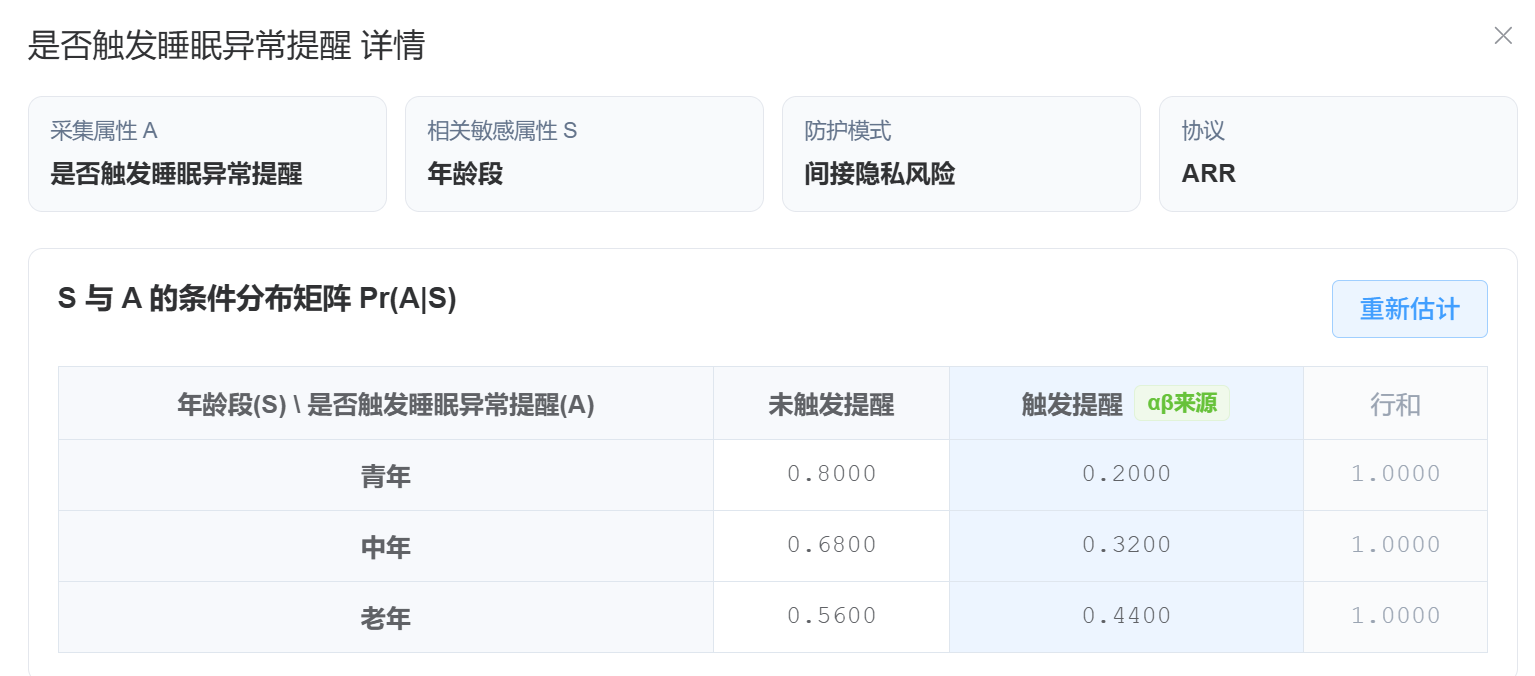
\includegraphics[width=\linewidth]{figures/ARR-估计条件分布矩阵.png}
  \\
  {\small (a) 条件分布矩阵}
\end{minipage}
\hfill
\begin{minipage}[b]{0.32\textwidth}
  \centering
  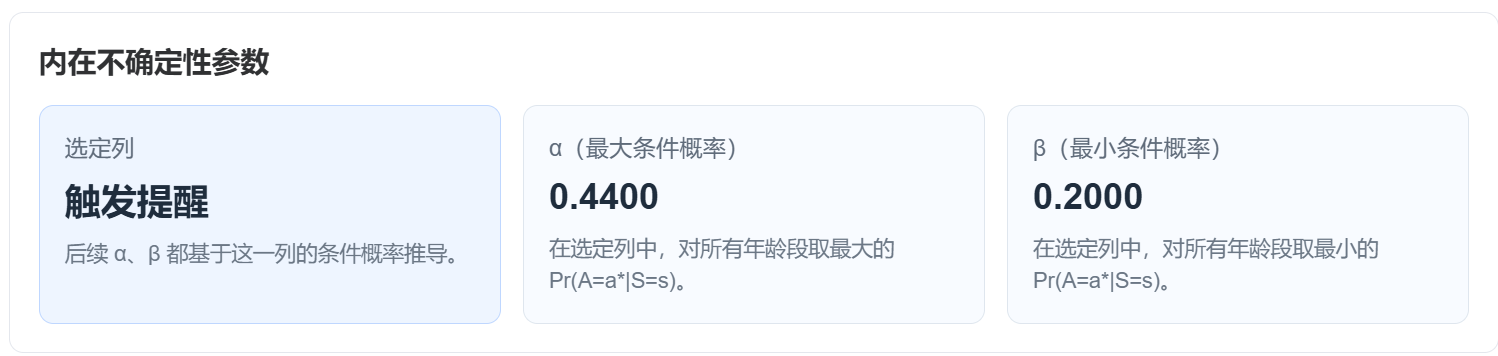
\includegraphics[width=\linewidth]{figures/ARR-计算内在不确定性参数.png}
  \\
  {\small (b) 内在不确定性参数}
\end{minipage}
\hfill
\begin{minipage}[b]{0.32\textwidth}
  \centering
  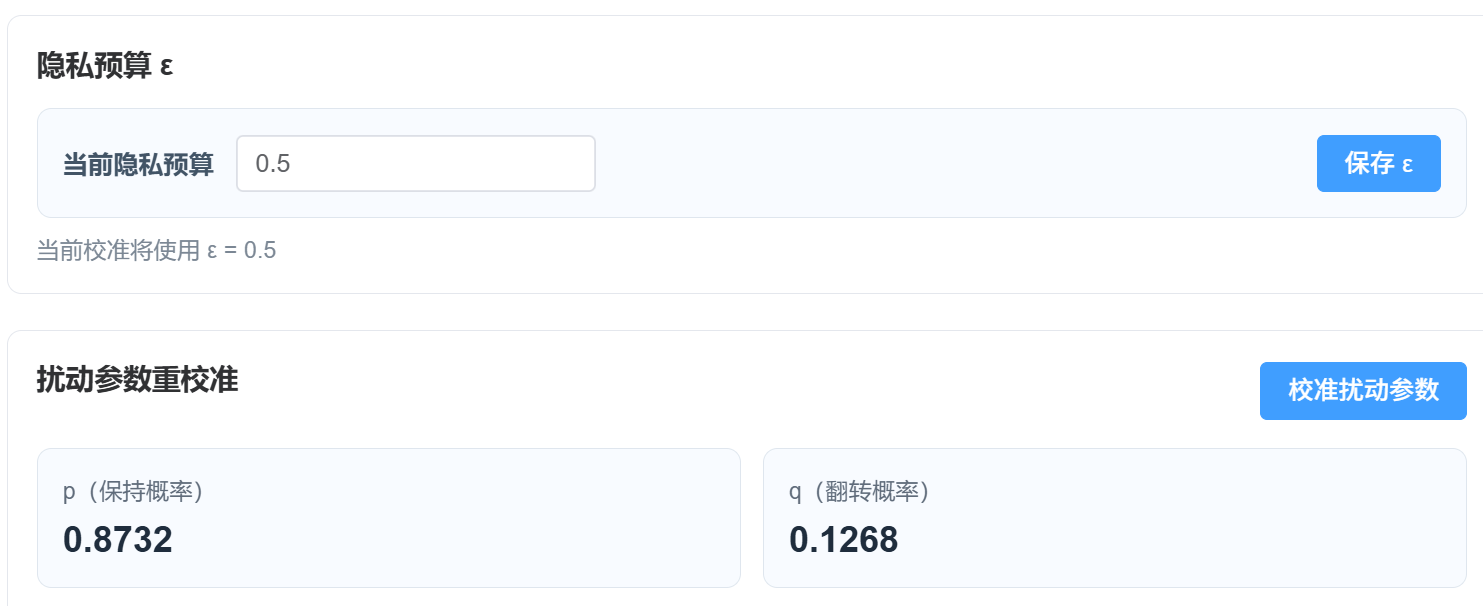
\includegraphics[width=\linewidth]{figures/ARR-扰动参数重校准.png}
  \\
  {\small (c) 扰动参数重校准}
\end{minipage}
\caption{ARR协议：管理端参数计算流程}
\end{figure}

客户端执行 ARR 协议时，先采集二值属性并完成编码，再根据管理端下发的扰动参数执行随机响应。由于该协议面向二值属性，编码结果较为直接，测试重点在于扰动后取值是否可能与原始取值不同，以及上传记录中是否保留任务编号、协议类型、隐私预算和扰动结果等必要信息。图中展示了从采集、编码到扰动的本地处理过程，说明原始值在上传前已经完成随机化保护。

\begin{figure}[htbp]
\centering
\begin{minipage}[b]{0.32\textwidth}
  \centering
  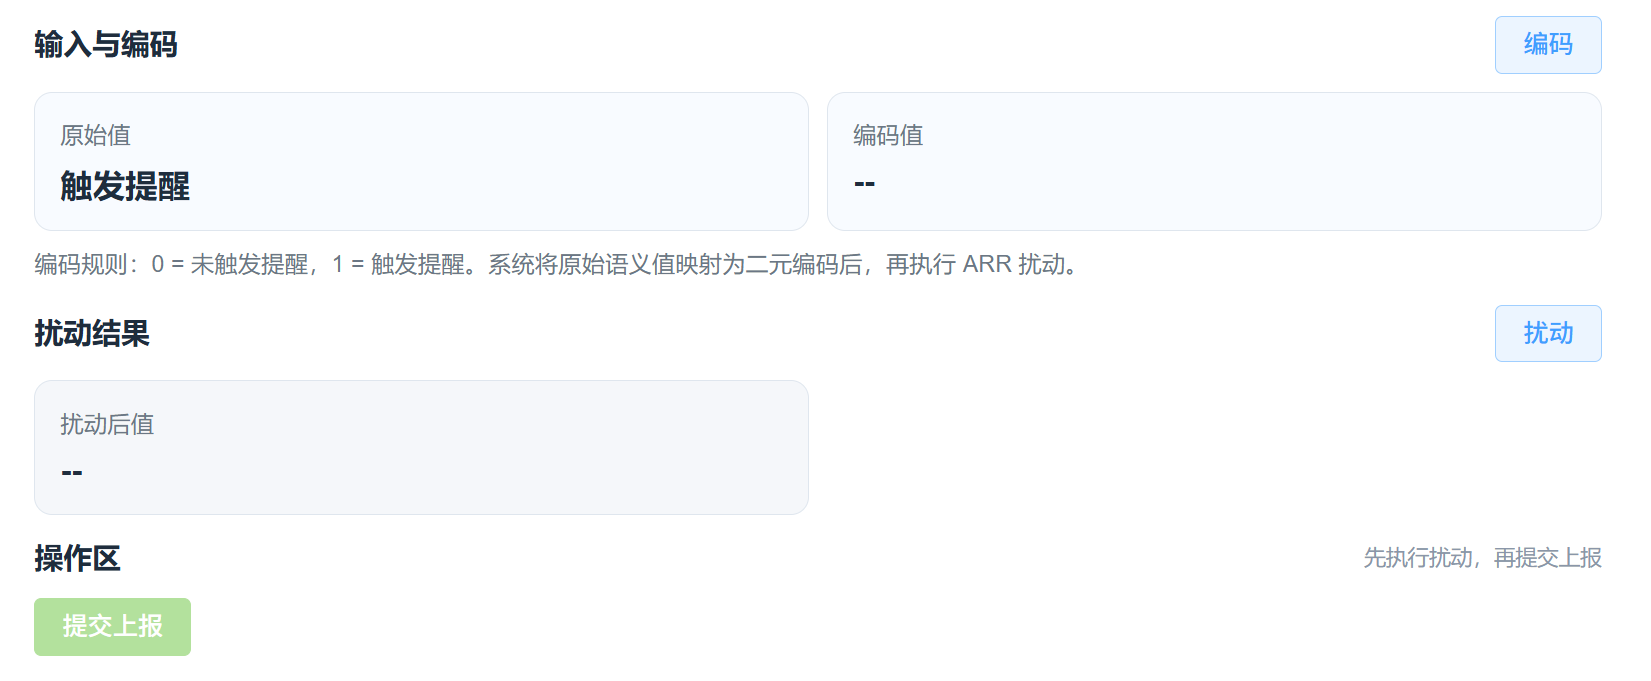
\includegraphics[width=\linewidth]{figures/ARR-采集.png}
  \\
  {\small (a) 采集}
\end{minipage}
\hfill
\begin{minipage}[b]{0.32\textwidth}
  \centering
  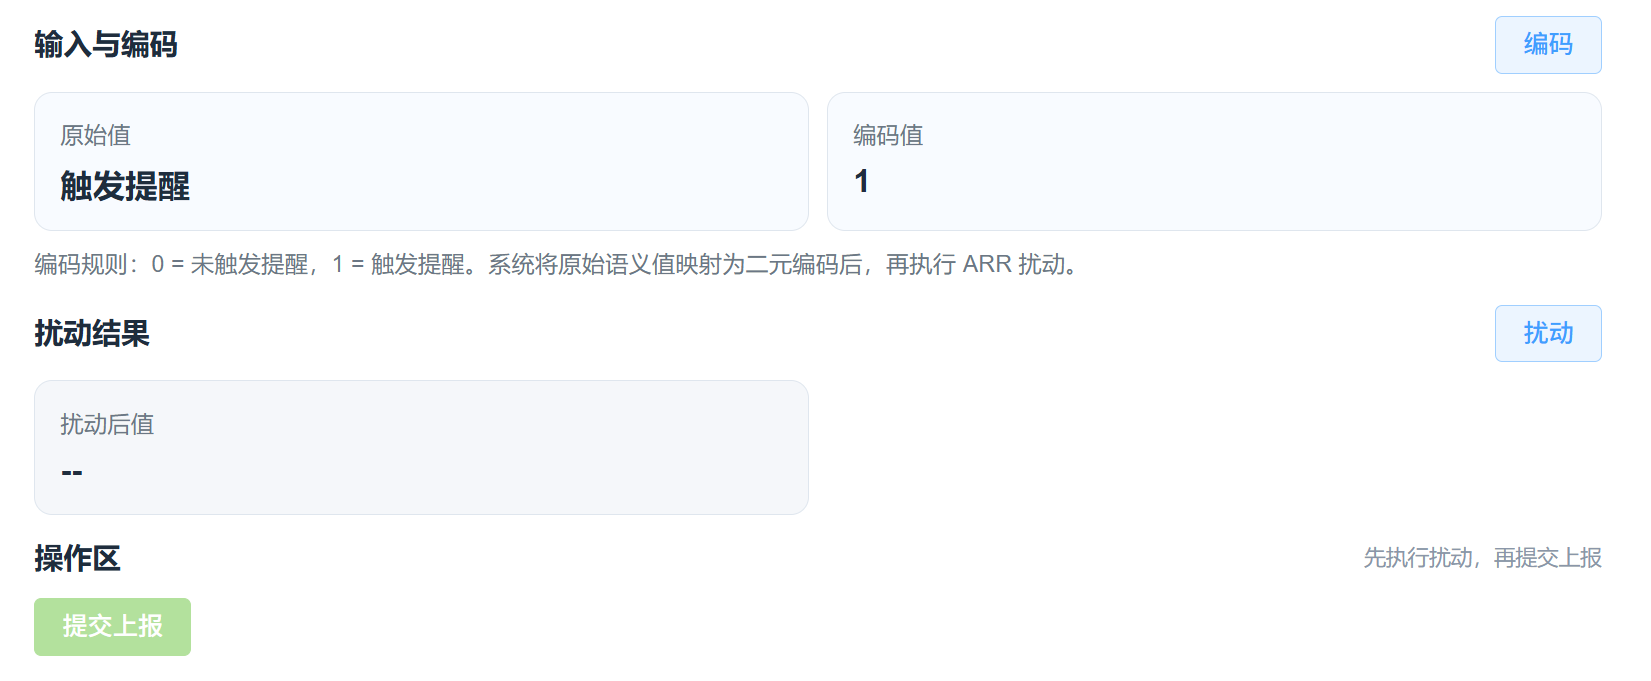
\includegraphics[width=\linewidth]{figures/ARR-编码.png}
  \\
  {\small (b) 编码}
\end{minipage}
\hfill
\begin{minipage}[b]{0.32\textwidth}
  \centering
  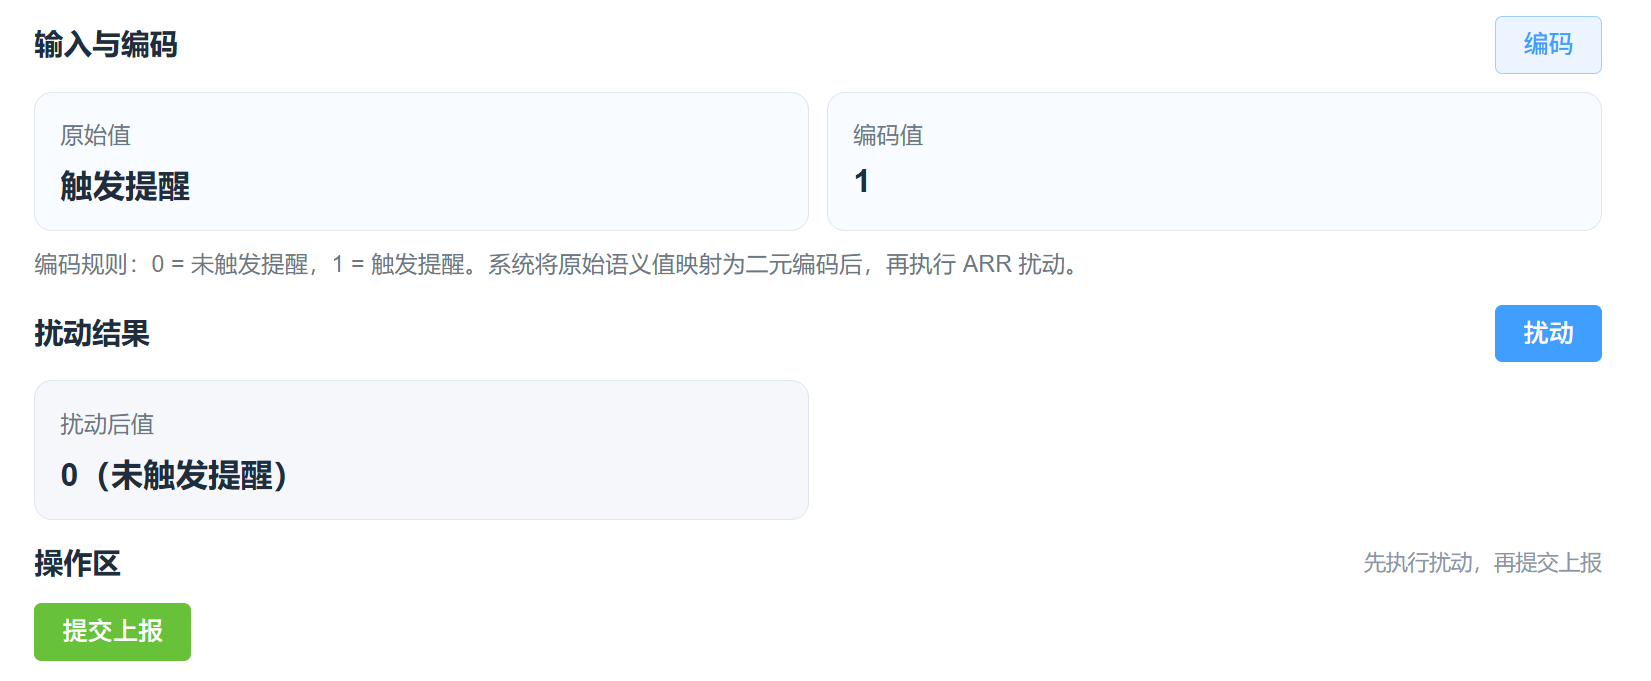
\includegraphics[width=\linewidth]{figures/ARR-扰动.png}
  \\
  {\small (c) 扰动}
\end{minipage}
\caption{ARR协议：客户端本地扰动与上传流程}
\end{figure}

在多客户端测试中，系统批量生成或接收多个客户端的扰动上报结果，并在管理端根据 ARR 的无偏估计公式恢复总体分布。聚合结果页面主要用于观察估计分布与真实分布是否保持相同趋势，以及在当前隐私预算下误差是否处于可接受范围。由于 ARR 的取值域只有两个类别，该部分适合用来验证系统从单次扰动到批量聚合的基础闭环。

\begin{figure}[htbp]
\centering
\begin{minipage}[b]{0.48\textwidth}
  \centering
  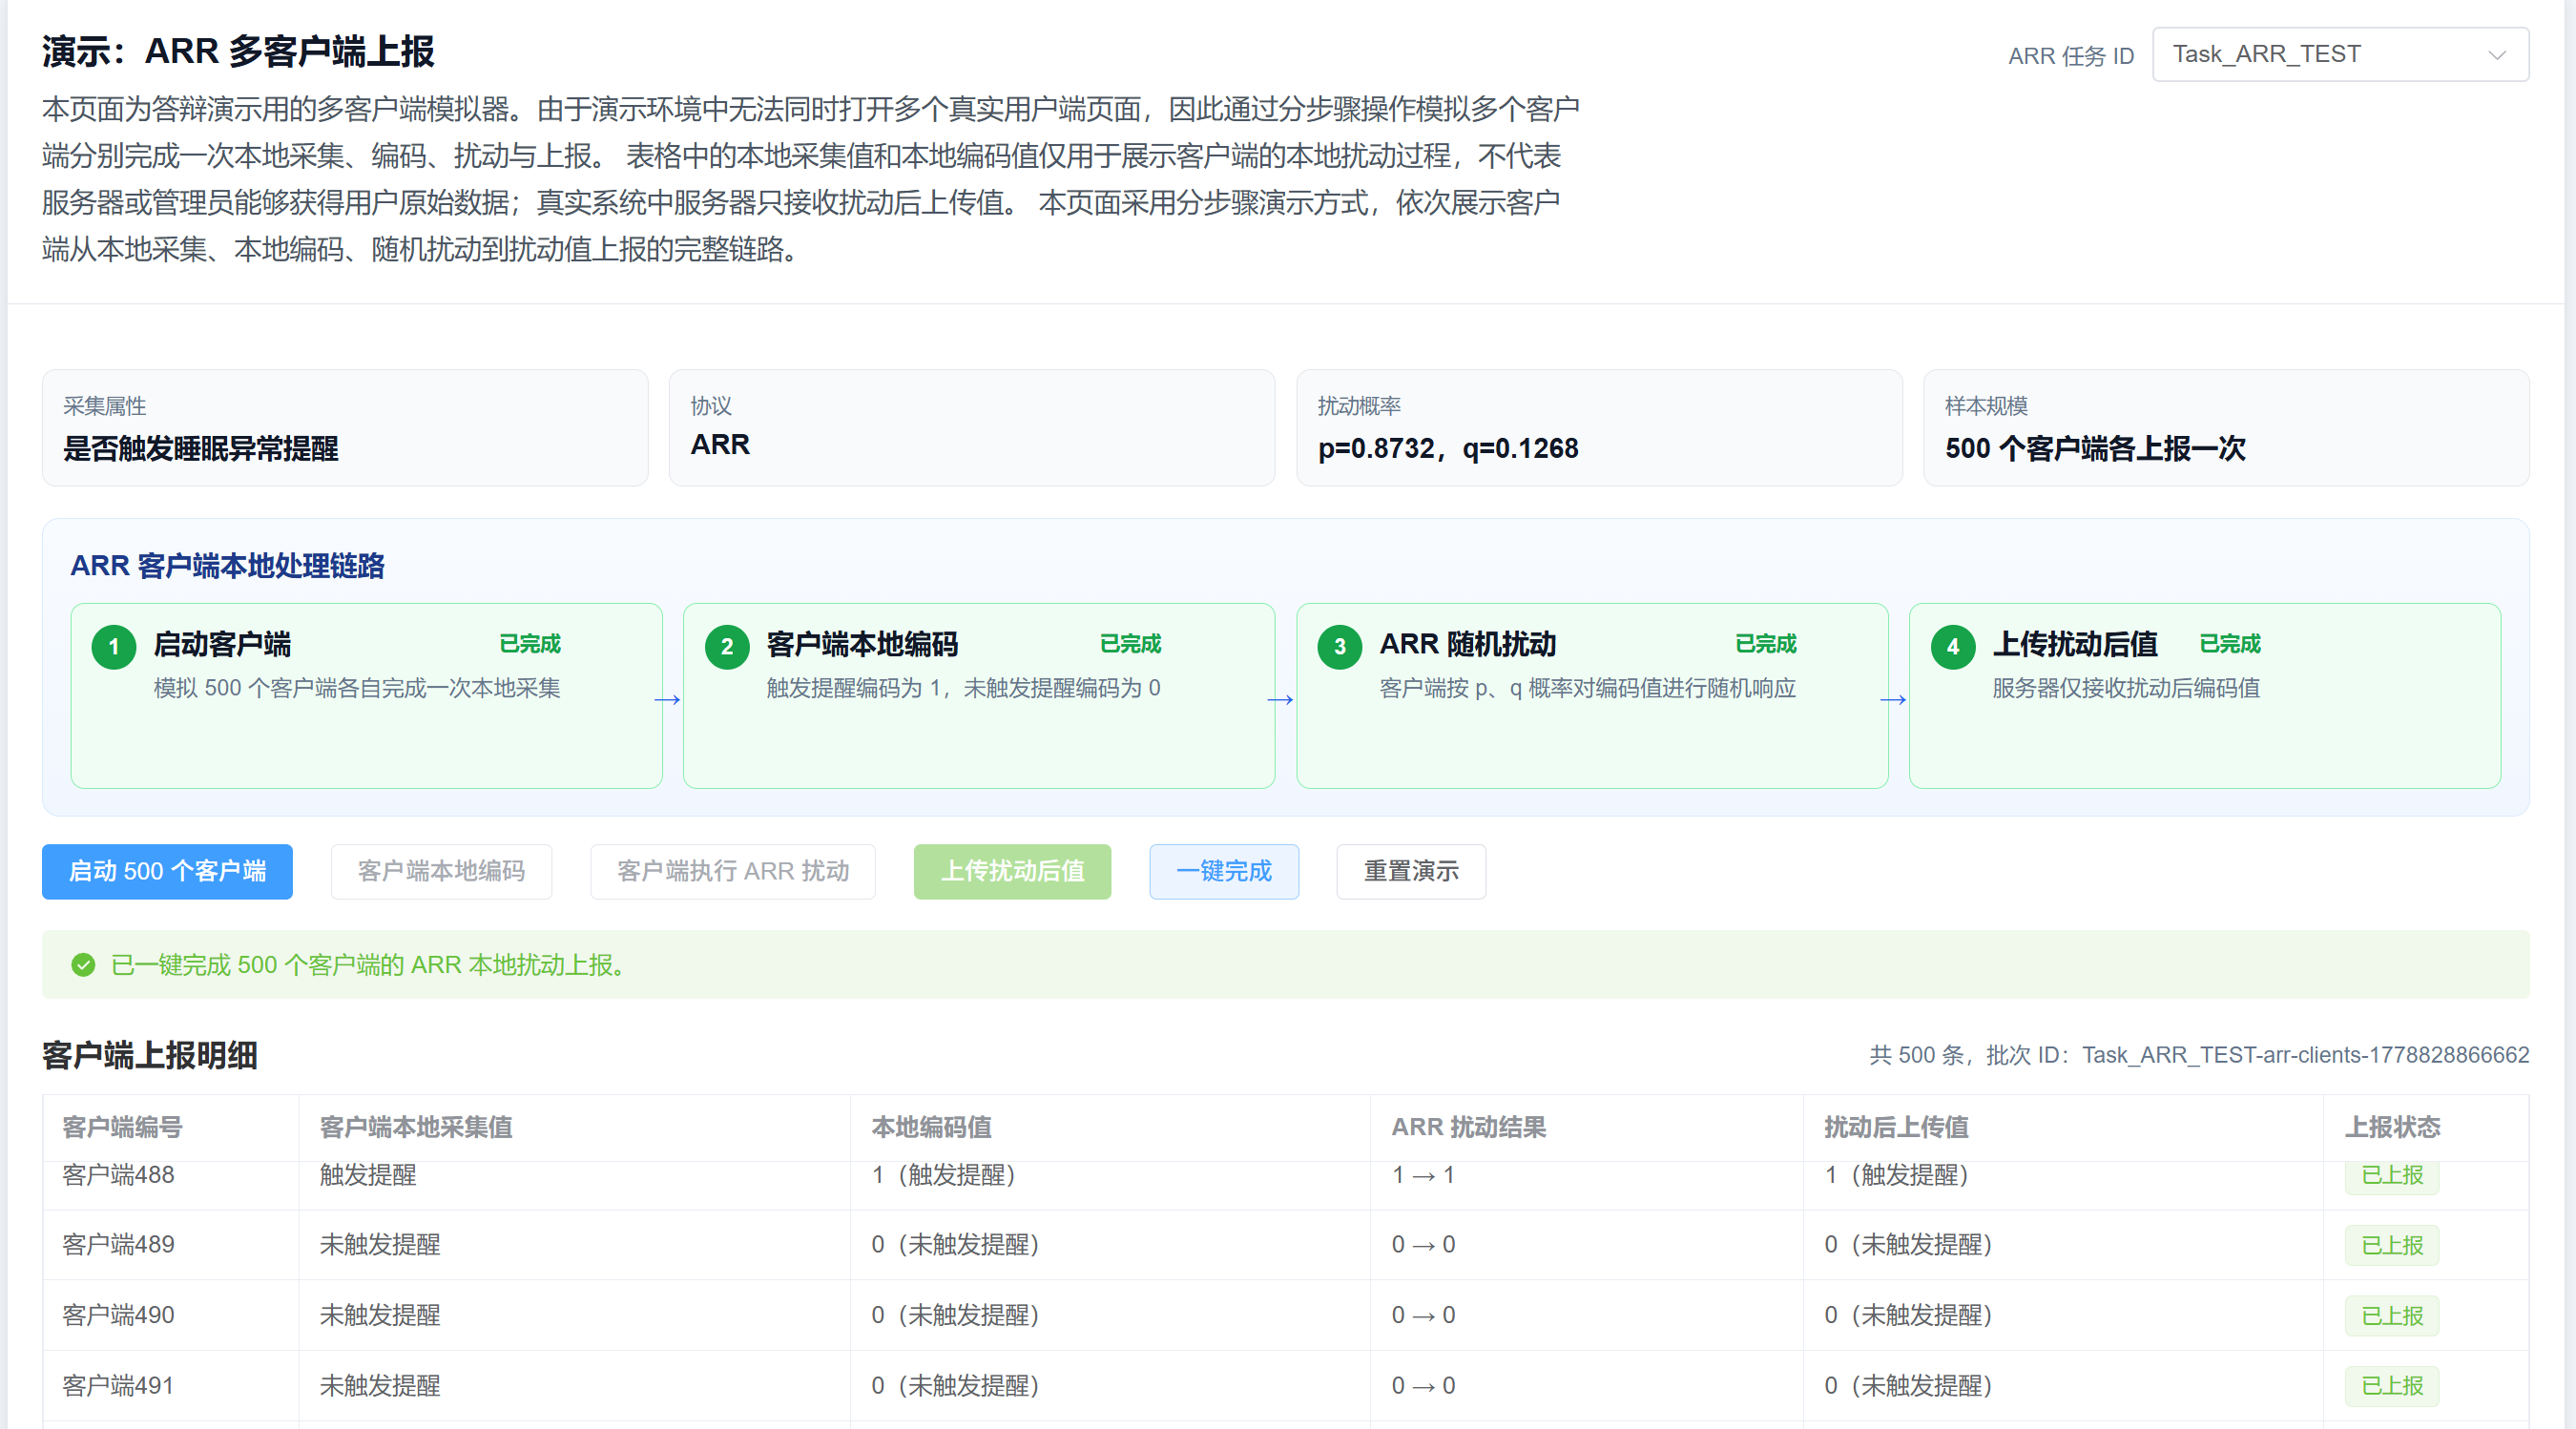
\includegraphics[width=\linewidth]{figures/ARR-多客户端上报.png}
  \\
  {\small (a) 多客户端上报}
\end{minipage}
\hfill
\begin{minipage}[b]{0.48\textwidth}
  \centering
  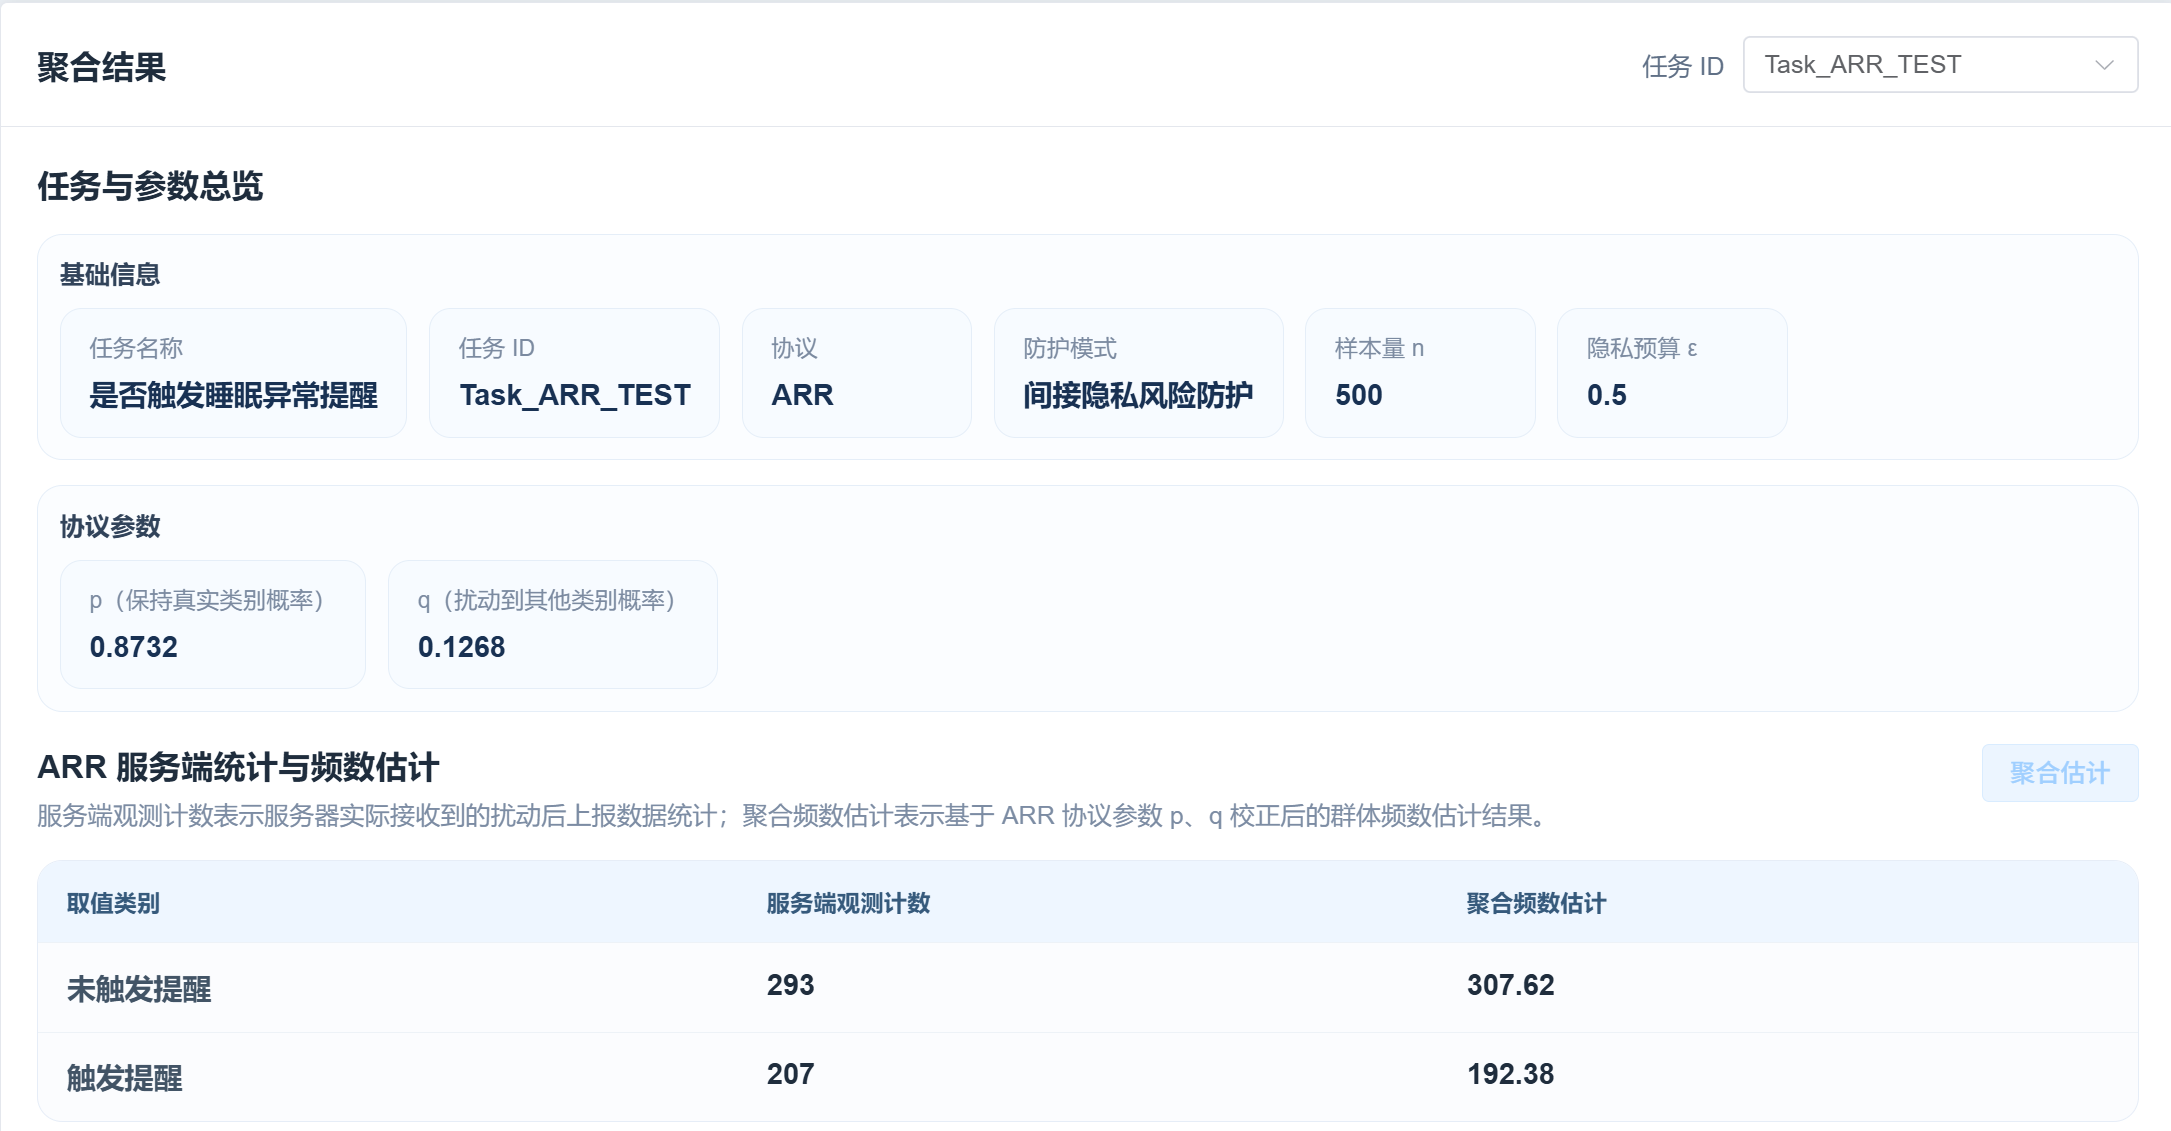
\includegraphics[width=\linewidth]{figures/ARR-聚合.png}
  \\
  {\small (c) 聚合结果}
\end{minipage}
\caption{ARR协议：多客户端上传与聚合结果展示}
\end{figure}

\begin{figure}[htbp]
\centering
\fbox{\parbox[c][0.22\textheight][c]{0.82\linewidth}{\centering ARR协议误差评估截图：可放置不同隐私预算下的 MSE、MAE 或真实/估计分布误差对比图}}
\caption{ARR协议：误差评估结果}
\end{figure}

\subsubsection{AGRR协议流程验证}

AGRR 协议面向具有条件分布关系的多值属性。系统先根据公开数据集估计条件分布矩阵，再计算内在不确定性，并在此基础上重校准扰动参数。与普通随机响应相比，AGRR 的流程多了条件分布估计和参数重校准环节，因此需要单独展示管理端参数计算过程以及客户端采集、编码、扰动过程。

在本测试场景中，AGRR 用于站立时长、活动等级等离散化后的多值属性。与 ARR 不同，AGRR 的取值域包含多个类别，因此系统需要同时考虑属性域大小 \(d\)、隐私预算 \(\varepsilon\) 以及条件分布所反映的间接泄露风险。管理端页面展示了从条件分布矩阵到 \(\alpha,\beta\) 参数，再到 \(p,q\) 扰动参数的完整计算过程。该过程可以验证系统是否能够针对不同多值字段生成不同的扰动策略，而不是对所有属性套用同一组固定参数。

\begin{figure}[htbp]
\centering
\begin{minipage}[b]{0.32\textwidth}
  \centering
  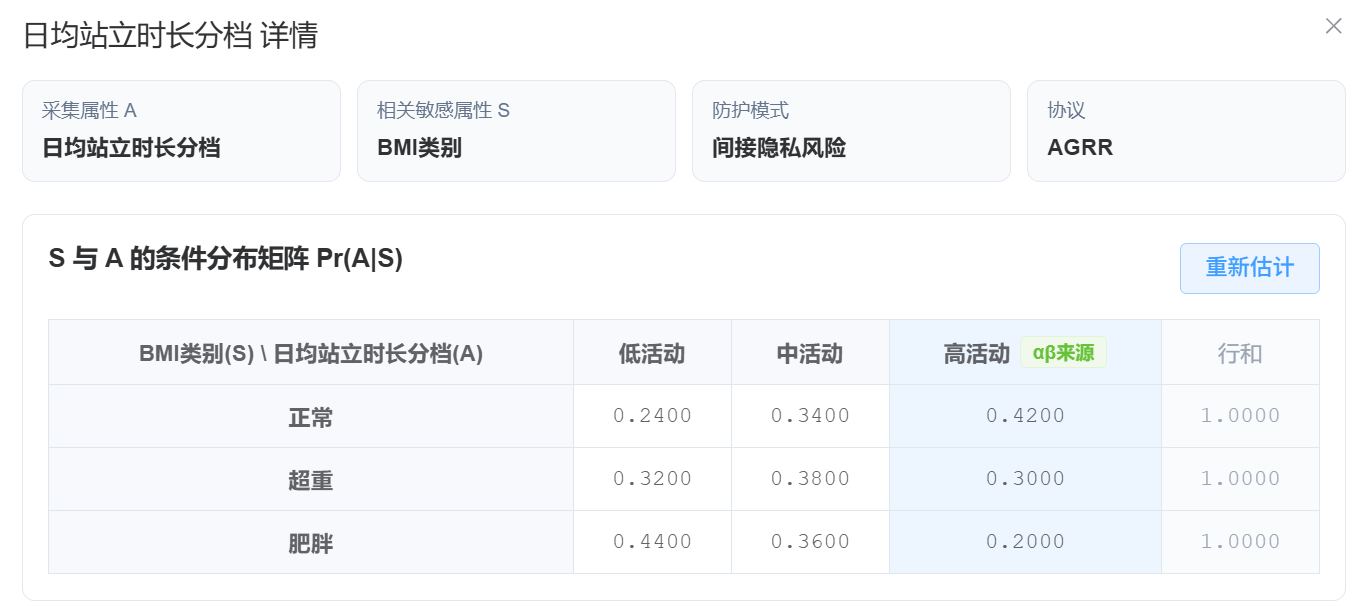
\includegraphics[width=\linewidth]{figures/AGRR-估计条件分布矩阵.png}
  \\
  {\small (a) 条件分布矩阵}
\end{minipage}
\hfill
\begin{minipage}[b]{0.32\textwidth}
  \centering
  
\includegraphics[width=\linewidth]{figures/AGRR-计算内在不确定性参数.png}
  \\
  {\small (b) 内在不确定性参数}
\end{minipage}
\hfill
\begin{minipage}[b]{0.32\textwidth}
  \centering
  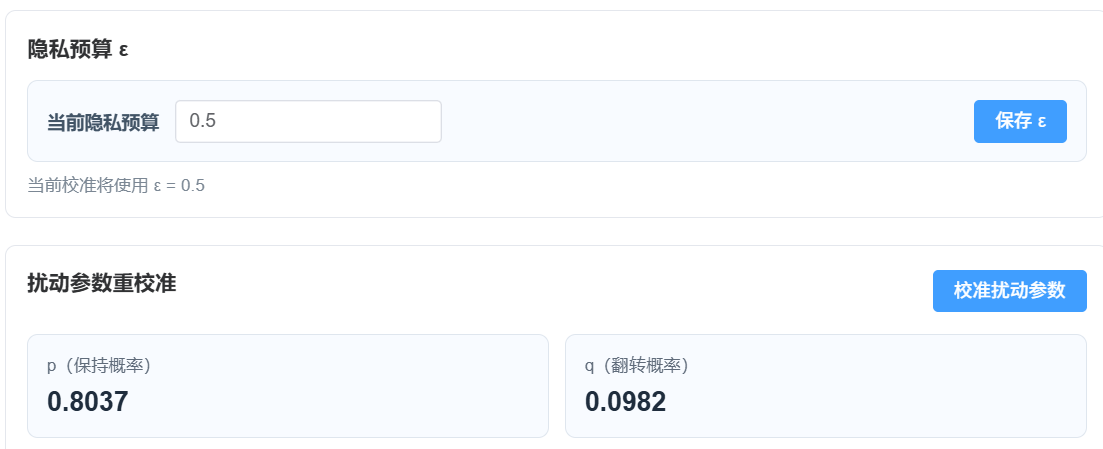
\includegraphics[width=\linewidth]{figures/AGRR-扰动参数重校准.png}
  \\
  {\small (c) 扰动参数重校准}
\end{minipage}
\caption{AGRR协议：管理端参数计算流程}
\end{figure}

客户端侧的 AGRR 测试主要关注多值属性的采集、编码和扰动是否保持一致。用户端首先将输入值映射到预设属性域中的某一类别，然后按照 AGRR 扰动规则以概率 \(p\) 保留原值，或以概率 \(q\) 上报其他类别。图中展示了客户端本地处理的关键步骤，能够说明多值字段在上报前已经经过随机扰动，管理端无法直接获得用户原始取值。

\begin{figure}[htbp]
\centering
\begin{minipage}[b]{0.32\textwidth}
  \centering
  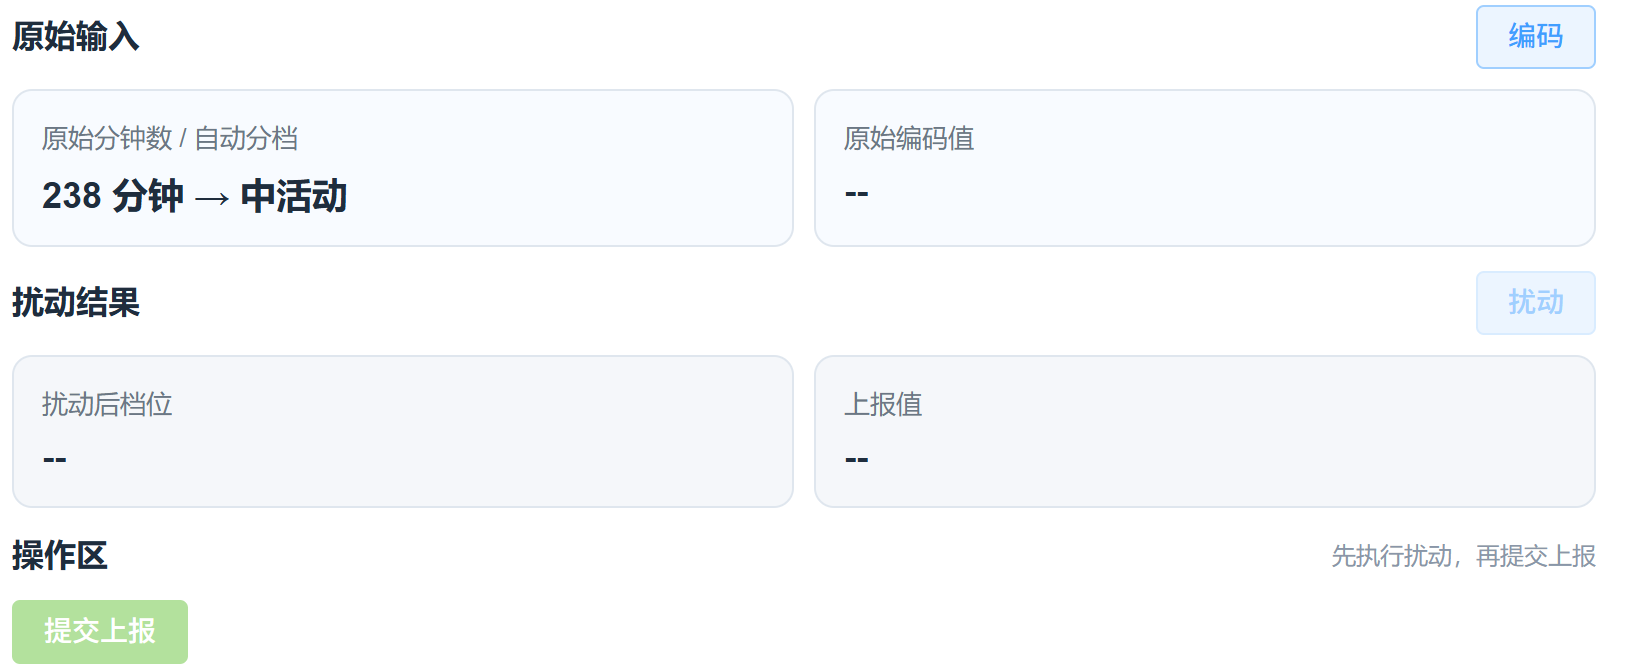
\includegraphics[width=\linewidth]{figures/AGRR-采集.png}
  \\
  {\small (a) 采集}
\end{minipage}
\hfill
\begin{minipage}[b]{0.32\textwidth}
  \centering
  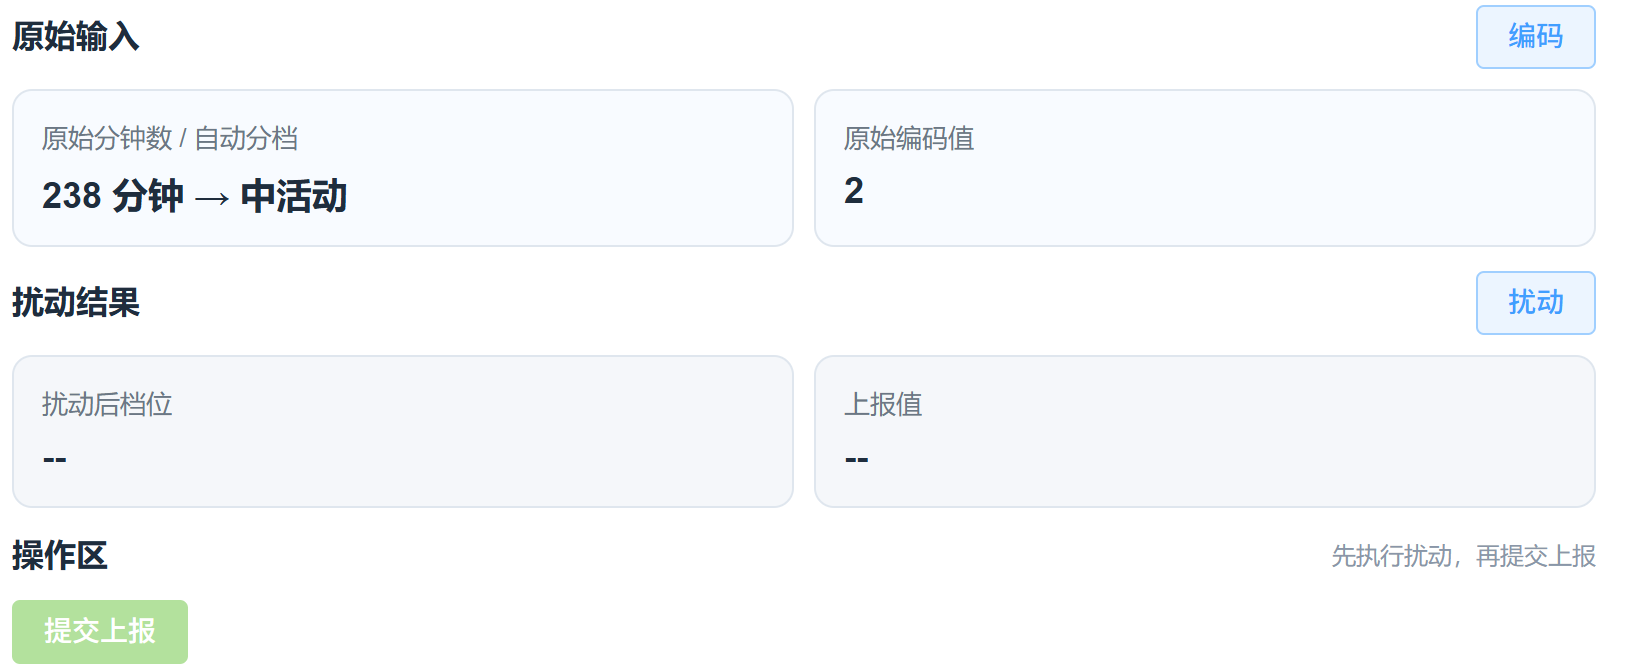
\includegraphics[width=\linewidth]{figures/AGRR-编码.png}
  \\
  {\small (b) 编码}
\end{minipage}
\hfill
\begin{minipage}[b]{0.32\textwidth}
  \centering
  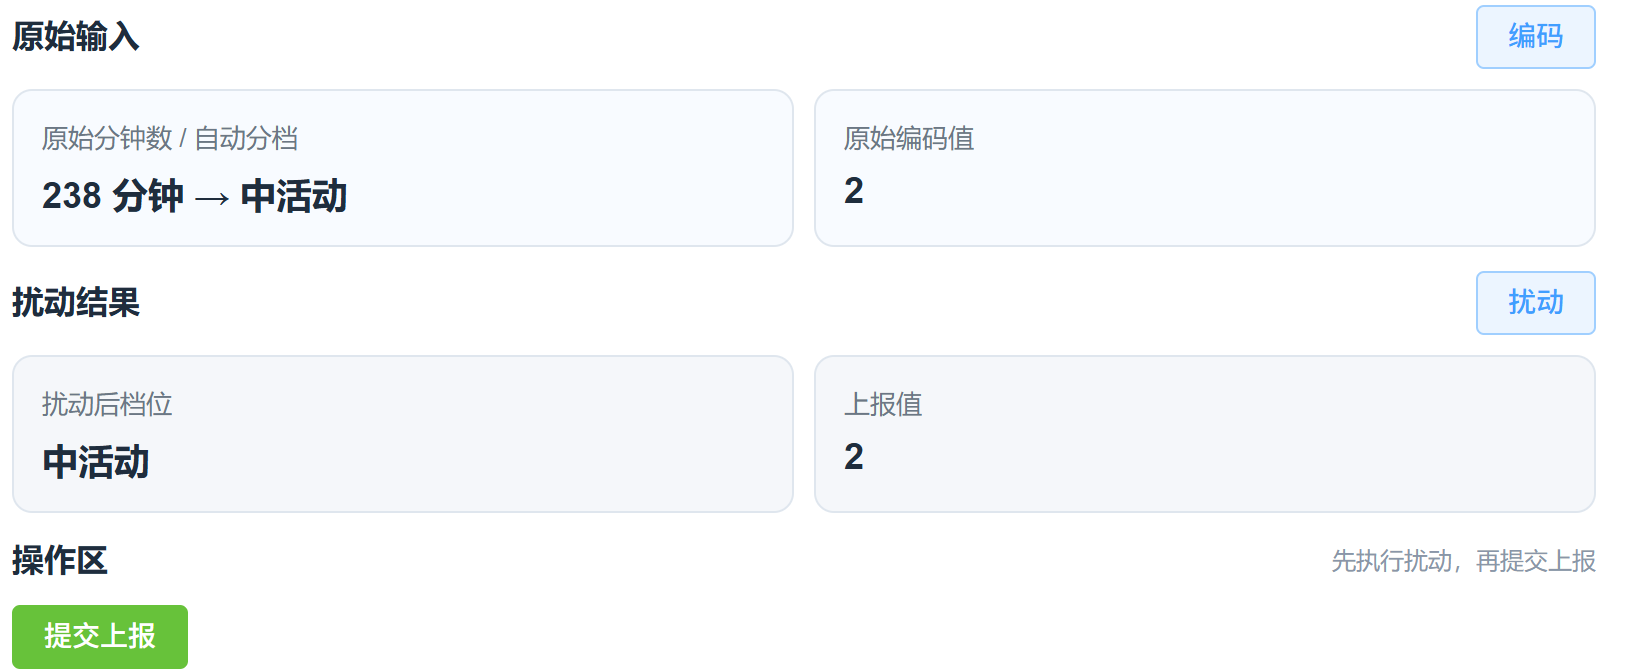
\includegraphics[width=\linewidth]{figures/AGRR-扰动.png}
  \\
  {\small (c) 扰动}
\end{minipage}
\caption{AGRR协议：客户端本地扰动与上传流程}
\end{figure}

在多客户端上传测试中，AGRR 的聚合页面用于验证系统能否统计各类别的扰动后上报次数，并通过无偏估计恢复多类别频数。相较 ARR，AGRR 的误差更容易受到取值域大小和样本规模影响，因此聚合图表不仅需要展示真实分布与估计分布的对比，也需要结合后续误差评估截图说明不同参数设置下的稳定性。

\begin{figure}[htbp]
\centering
\begin{minipage}[b]{0.48\textwidth}
  \centering
  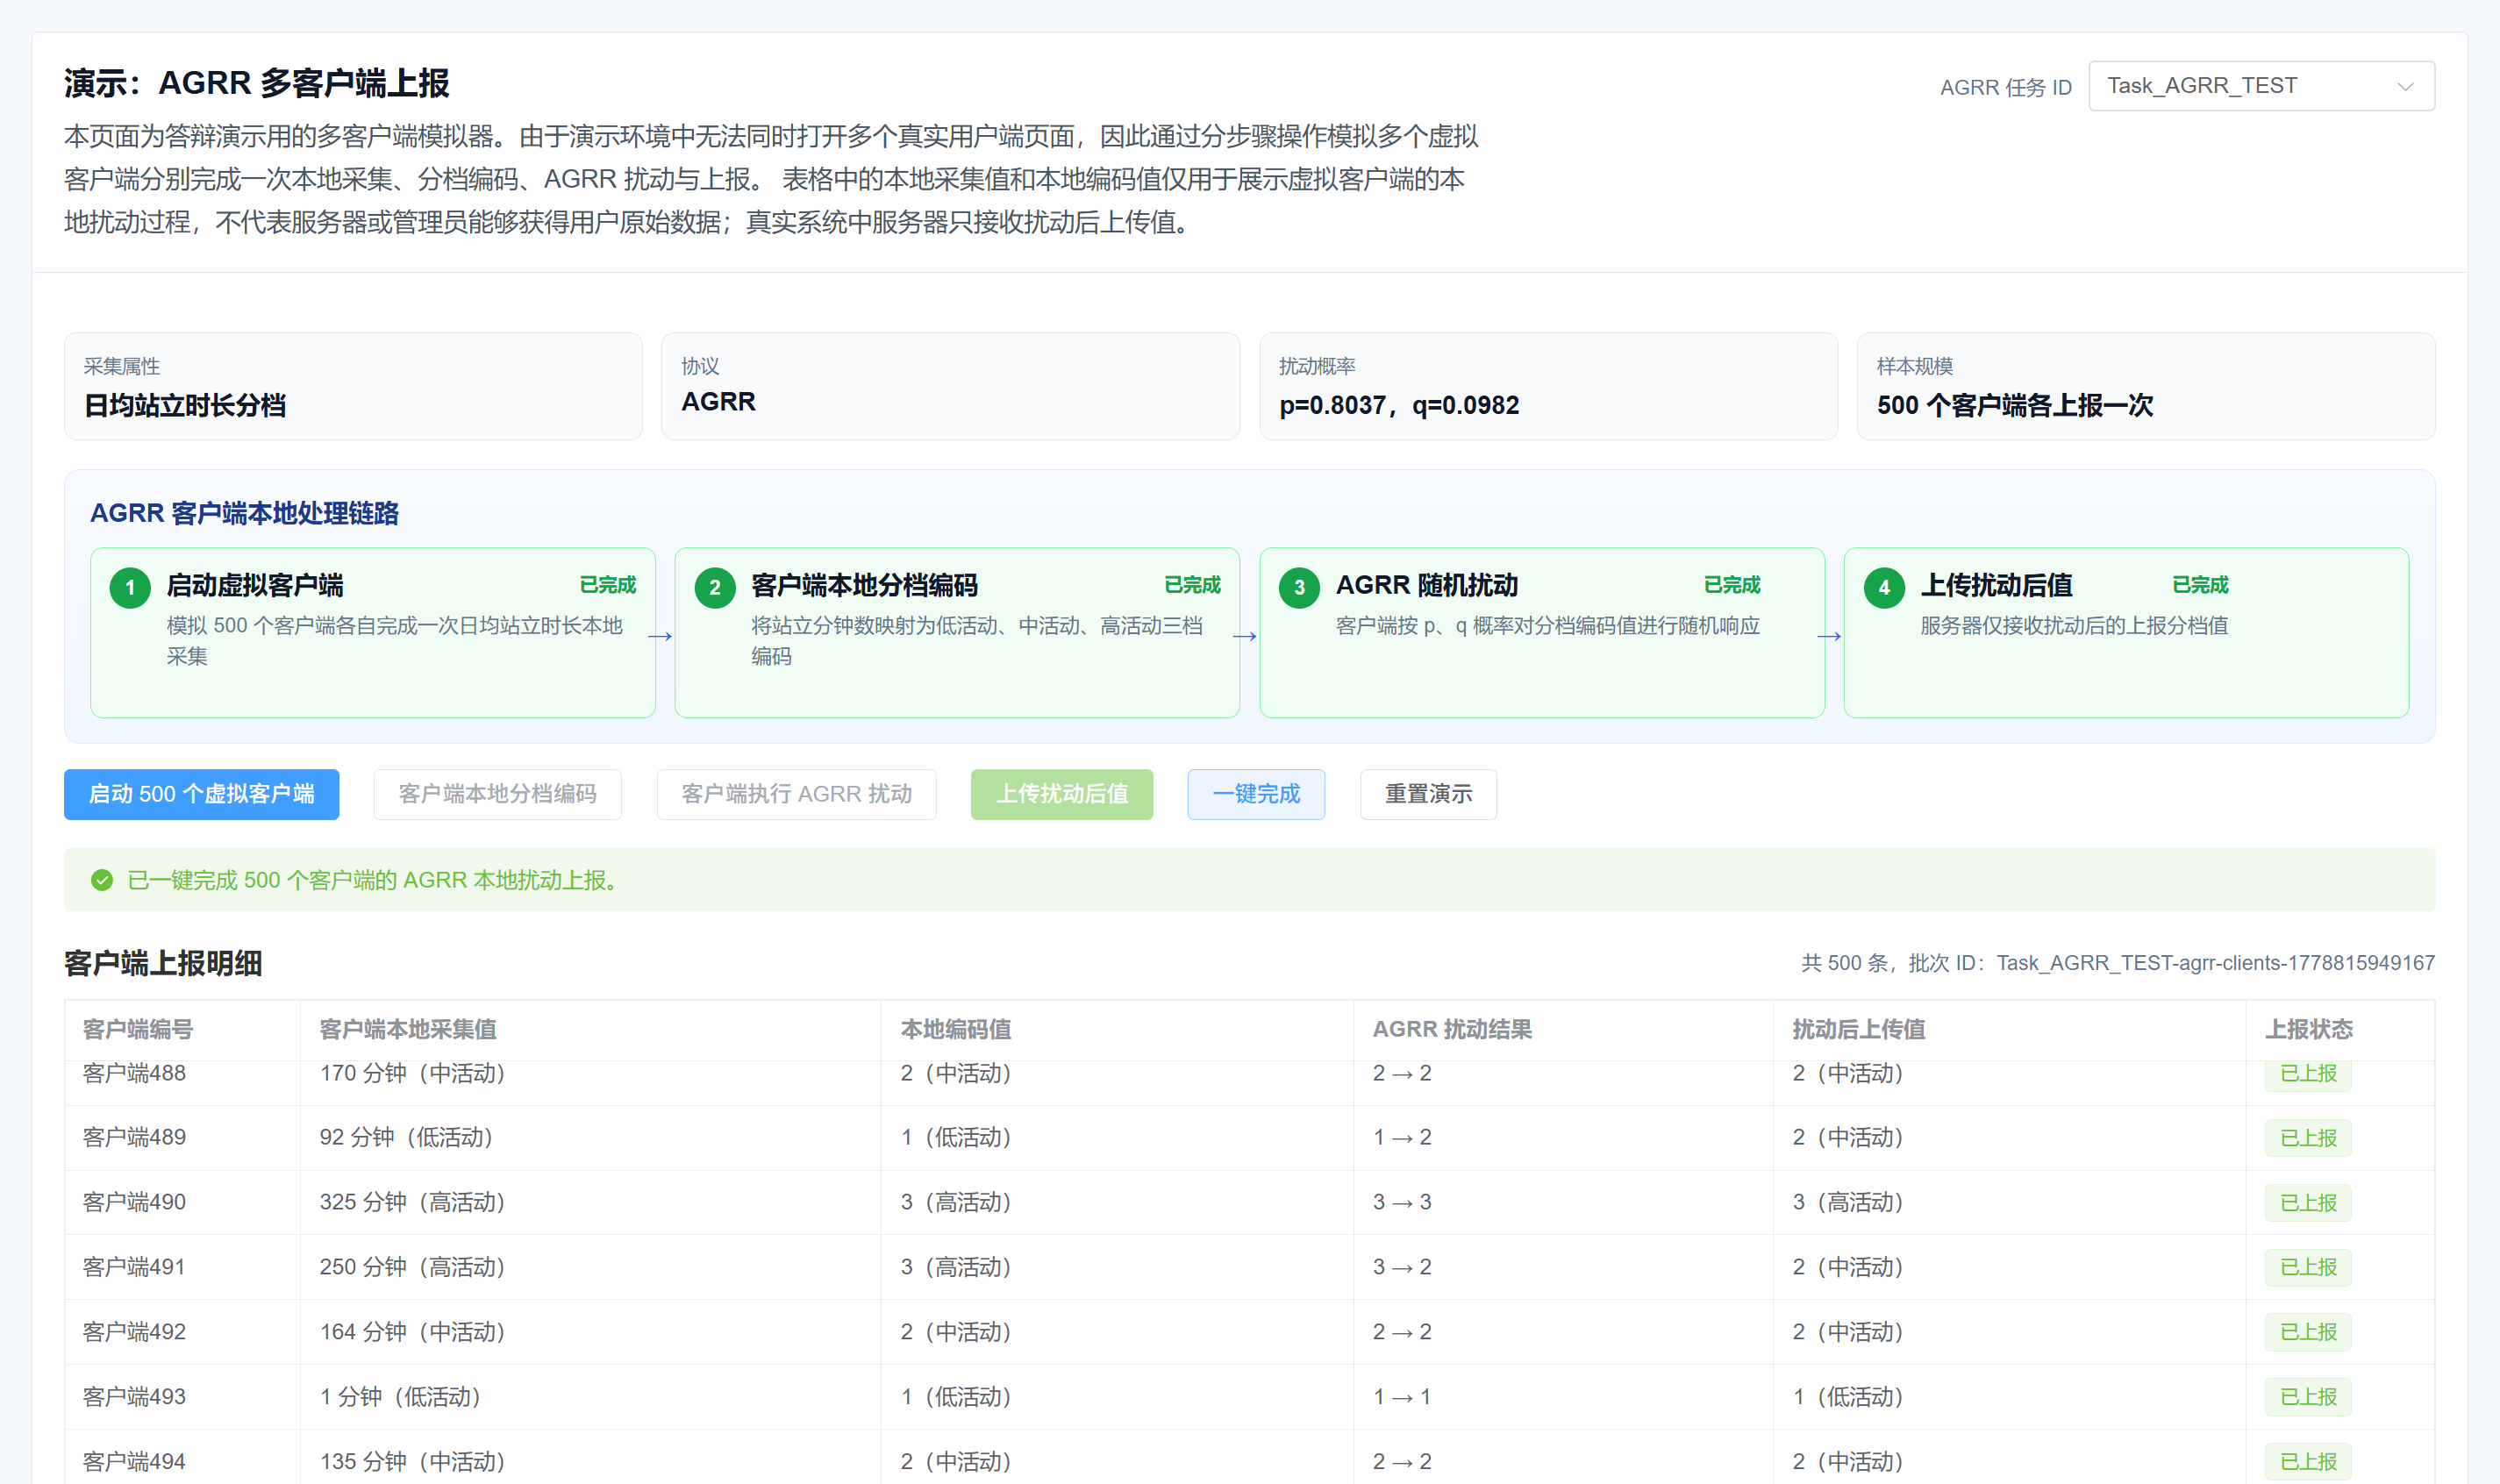
\includegraphics[width=\linewidth]{figures/AGRR-多客户端上报.png}
  \\
  {\small (a) 多客户端上报}
\end{minipage}
\hfill
\begin{minipage}[b]{0.48\textwidth}
  \centering
  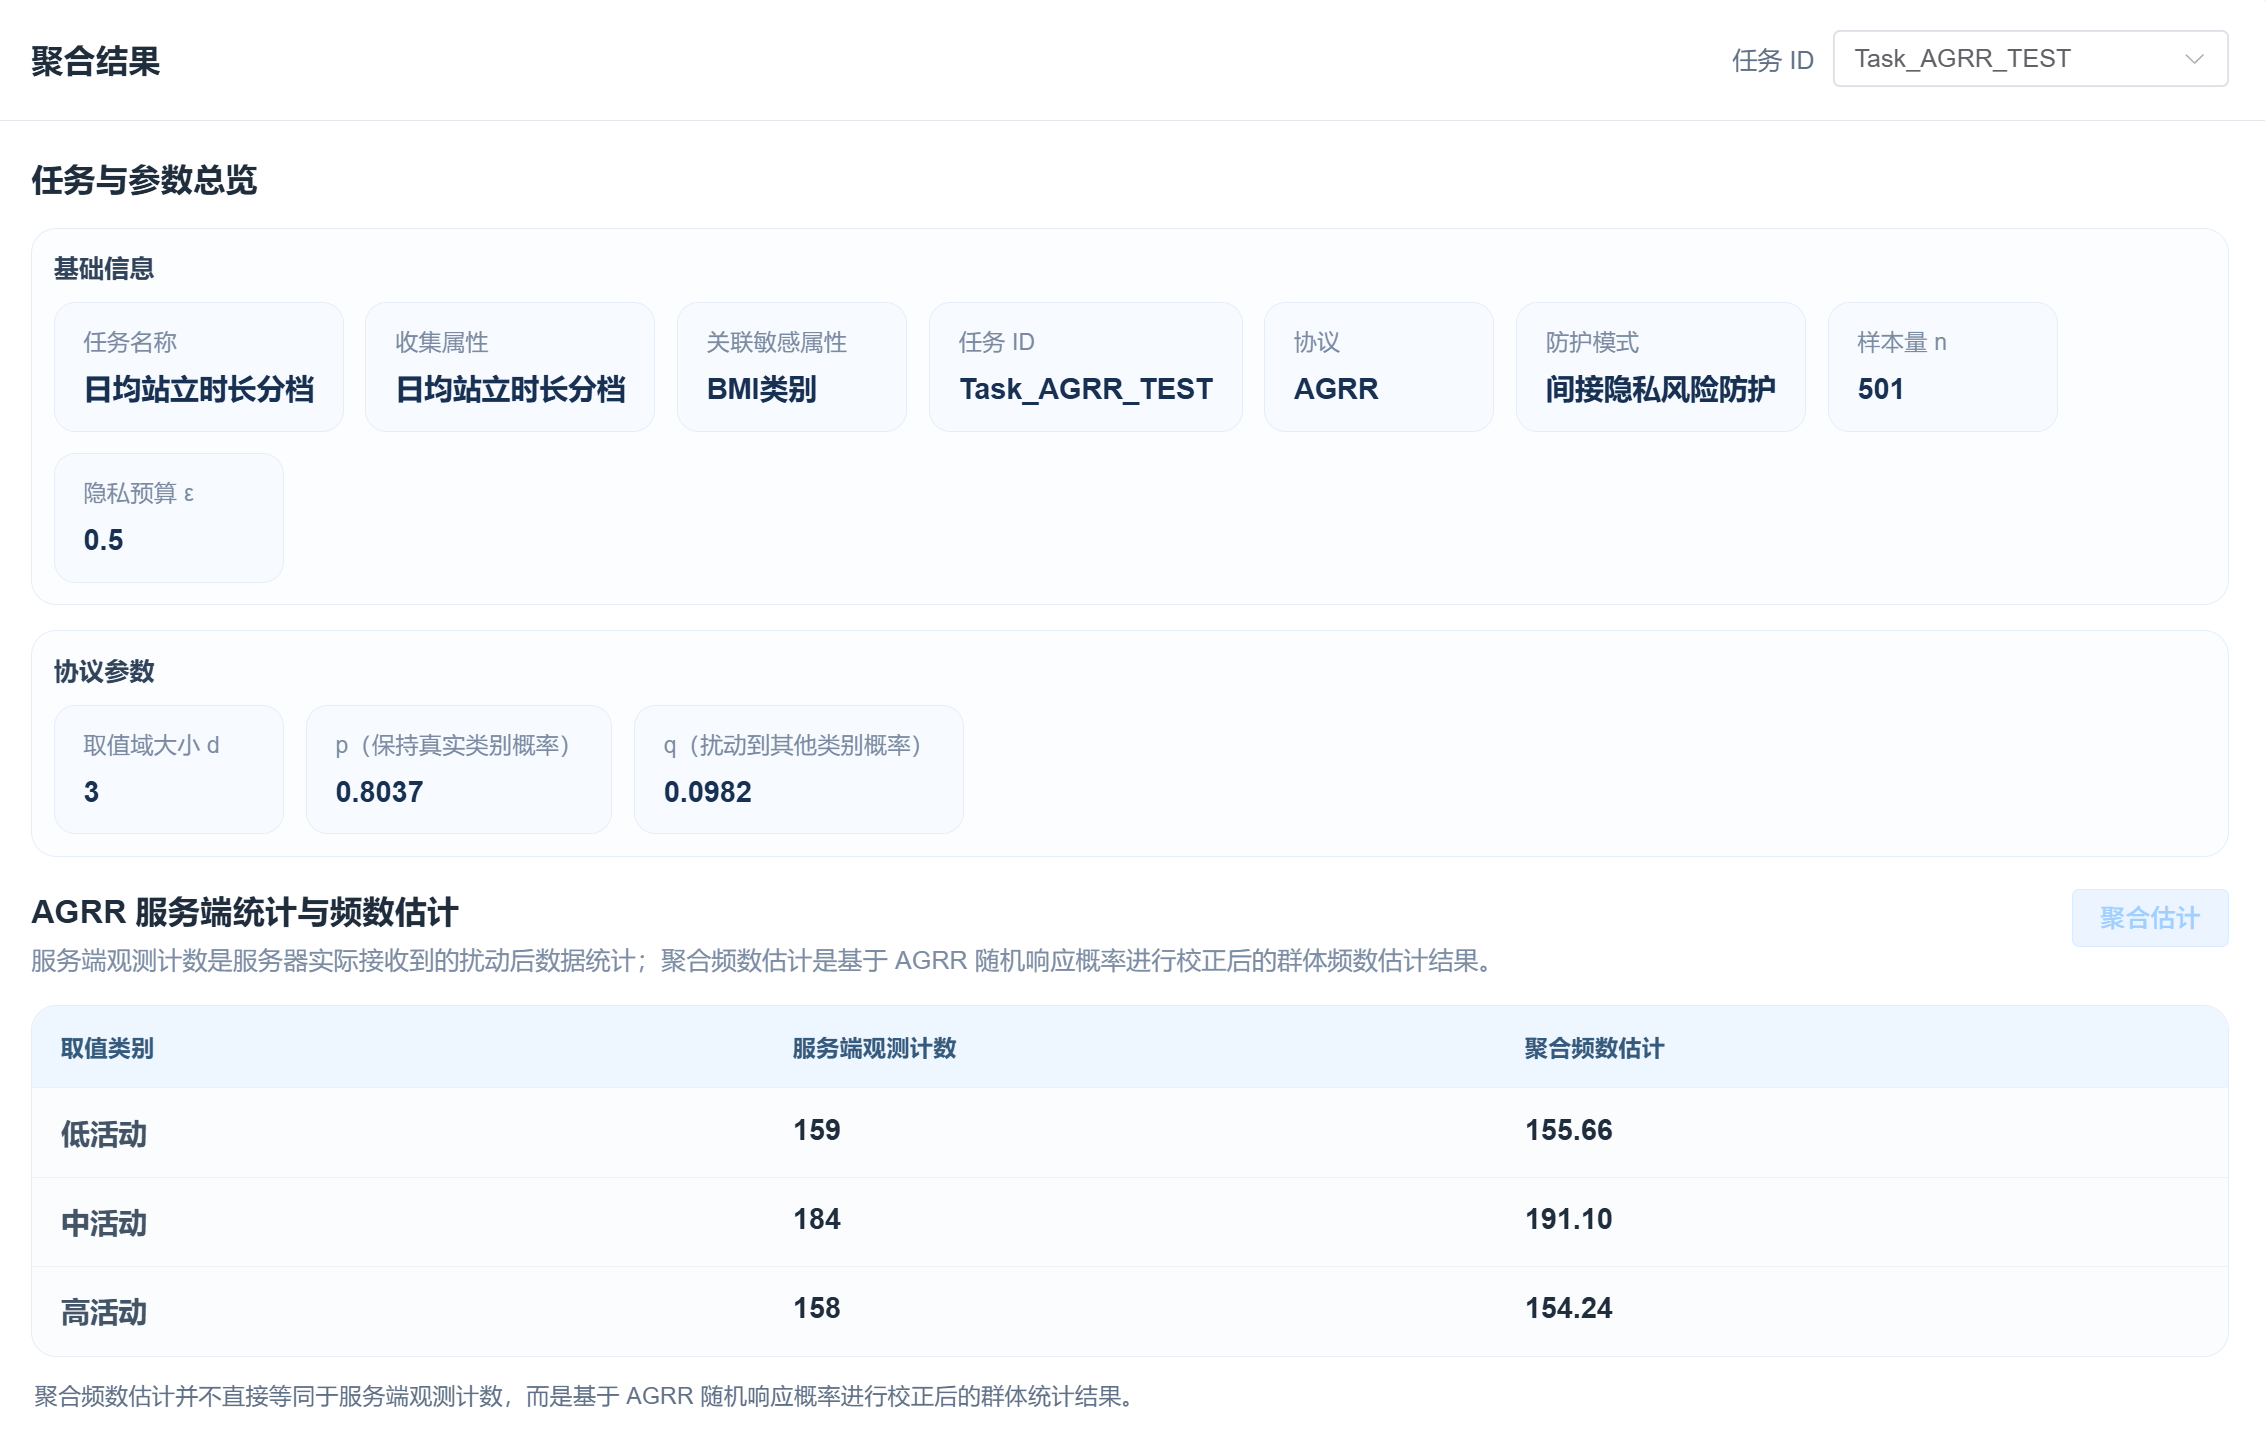
\includegraphics[width=\linewidth]{figures/AGRR-聚合.png}
  \\
  {\small (c) 聚合结果}
\end{minipage}
\caption{AGRR协议：多客户端上传与聚合结果展示}
\end{figure}

\begin{figure}[htbp]
\centering
\fbox{\parbox[c][0.22\textheight][c]{0.82\linewidth}{\centering AGRR协议误差评估截图：可放置多值属性在不同 \(\varepsilon\)、不同样本批次下的 MSE、MAE 对比图}}
\caption{AGRR协议：误差评估结果}
\end{figure}

\subsubsection{AOUE协议流程验证}

AOUE 协议主要用于取值域较大的离散属性，例如步数分桶、活动等级或其他多类别行为字段。该协议需要先将原始类别转换为一元编码向量，再对向量中的每一位进行随机扰动，因此测试时应重点展示属性域配置、一元编码结果、扰动向量上传以及服务端频率估计结果。

\begin{figure}[htbp]
\centering
\begin{minipage}[b]{0.32\textwidth}
  \centering
  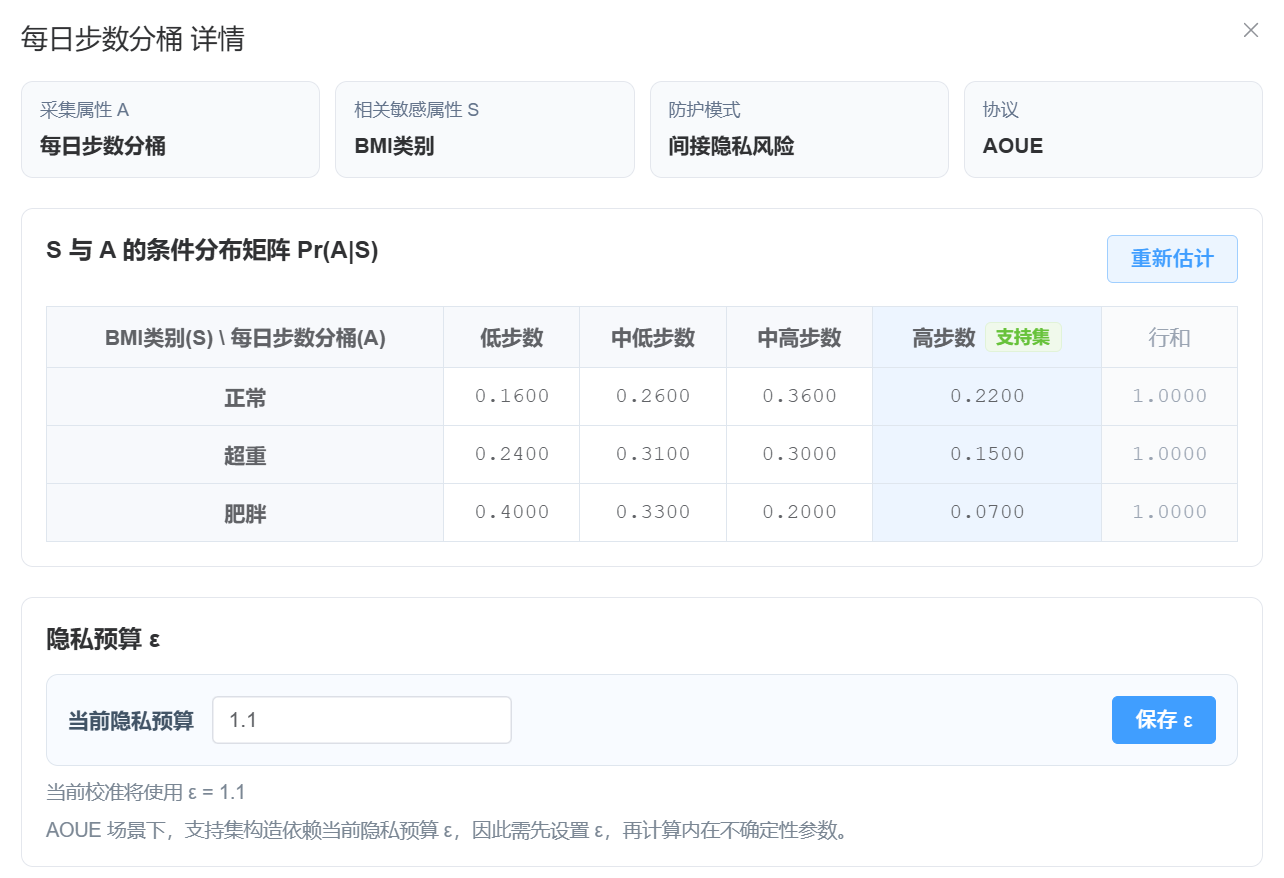
\includegraphics[width=\linewidth]{figures/AOUE-估计条件分布矩阵.png}
  \\
  {\small (a) 条件分布矩阵}
\end{minipage}
\hfill
\begin{minipage}[b]{0.32\textwidth}
  \centering
  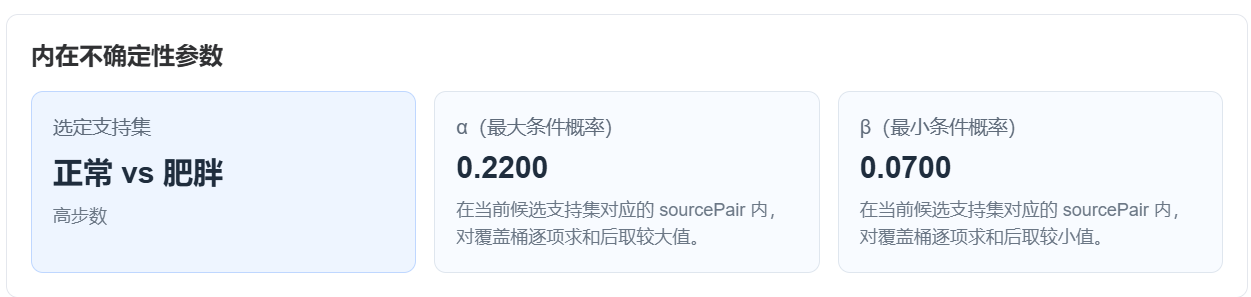
\includegraphics[width=\linewidth]{figures/AOUE-计算内在不确定性参数.png}
  \\
  {\small (b) 内在不确定性参数}
\end{minipage}
\hfill
\begin{minipage}[b]{0.32\textwidth}
  \centering
  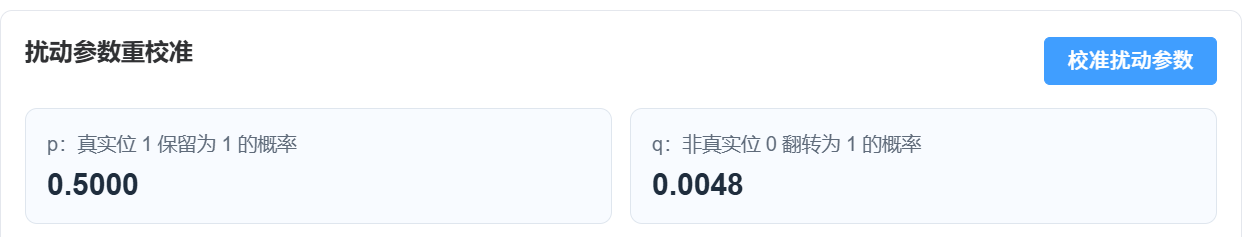
\includegraphics[width=\linewidth]{figures/AOUE-扰动参数重校准.png}
  \\
  {\small (c) 扰动参数重校准}
\end{minipage}
\caption{AOUE协议：管理端参数计算流程}
\end{figure}

\subsubsection{TSP协议流程验证}

TSP 协议用于混合隐私风险场景，即同一字段中既可能包含直接敏感取值，也可能包含与敏感属性相关的非敏感取值。该协议的流程需要先区分敏感取值集合和非敏感取值集合，再分别执行两阶段扰动与上报，因此测试时应重点展示字段分类、两阶段扰动结果以及最终聚合统计结果。

\begin{figure}[htbp]
\centering
\fbox{\parbox[c][0.22\textheight][c]{0.82\linewidth}{\centering TSP敏感/非敏感取值划分与参数配置截图}}
\caption{TSP协议：取值集合划分与参数配置}
\end{figure}

\begin{figure}[htbp]
\centering
\fbox{\parbox[c][0.22\textheight][c]{0.82\linewidth}{\centering TSP两阶段扰动上传与聚合结果截图}}
\caption{TSP协议：两阶段扰动上传与聚合结果展示}
\end{figure}

\begin{figure}[htbp]
\centering
\fbox{\parbox[c][0.22\textheight][c]{0.82\linewidth}{\centering TSP协议误差评估截图：可放置缺失值比例估计、非缺失取值估计以及两阶段扰动总体误差图}}
\caption{TSP协议：误差评估结果}
\end{figure}

\subsection{隐私保护算法实验与对比}

\subsubsection{ARR 算法测试}

\subsubsection{AOUE 算法测试}

\subsubsection{AGRR 算法测试}

\subsubsection{TSP 算法测试}

\subsection{测试结果分析}

\subsubsection{功能完整性分析}

\subsubsection{聚合精度分析}

\subsubsection{不同隐私预算下的结果对比}

\subsubsection{不同算法的性能对比}

\subsubsection{系统稳定性与可用性分析}

\subsection{本章小结}

\section{创新性说明}

本章围绕“风险如何度量、协议如何设计、系统如何落地”三个层次说明作品创新性。与专利说明书中的通用流程不同，本章以健康手环系统为表达对象，说明内在不确定性、本地扰动、参数重校准和混合隐私防护如何具体服务于睡眠、活动和夜间异常监测数据的隐私保护。

\subsection{创新点一：面向健康手环间接泄露风险的内在不确定性度量}

\subsubsection{现有技术的不足}

在健康手环数据采集中，平台往往不会直接询问用户是否存在心理健康风险、代谢风险或高 BMI 状态，而是收集睡眠和活动相关摘要。但这些摘要并非完全“无害”：睡眠碎片化等级可能与心理健康风险相关，步数分桶可能与代谢状态相关，站立时长分档可能与 BMI 类别相关。

传统做法通常有两种极端：一种是不加保护直接上传 A，这会放大间接推断风险；另一种是把所有 A 都当作完全敏感字段进行标准 LDP 扰动，这虽然保守，但会使低风险字段也承受高强度噪声，导致统计结果失真。例如，若睡眠时长状态与心理健康风险之间的条件分布差异很小，平台仍按最坏情况强噪声处理，就会牺牲本来可以保留的统计价值。

因此，本项目并不简单追求“加更多噪声”，而是关注一个更精细的问题：在既定隐私要求下，如何判断某个健康手环字段到底需要加多少噪声。这个判断不能只看字段取值个数，也不能完全依赖经验，而应当结合该字段与敏感属性之间的实际相关性。

\subsubsection{本作品的创新做法}

本作品将内在不确定性引入健康手环本地扰动参数设计中，用于量化“从非敏感属性 A 推断敏感属性 S 的天然难度”。系统首先根据样本数据、公开数据或合成数据设定条件分布 Pr(A|S)，再比较不同敏感状态下同一 A 取值出现概率的差异。

在本作品中，α 可以理解为某一 A 取值在不同 S 条件下的较高出现概率，β 可以理解为对应的较低出现概率。α/β 越接近 1，说明不同敏感群体中该 A 的出现概率越接近，A 对 S 的区分能力越弱；α/β 越大，说明该 A 在不同敏感群体中的分布差异越明显，间接推断风险越高。

以睡眠时长状态为例，如果“睡眠时长合理”在心理健康低风险和高风险群体中的出现概率接近，则攻击者难以仅凭该字段判断用户风险，系统可以降低扰动强度；以睡眠碎片化等级为例，如果“高碎片化”在不同风险群体中的出现概率差异较大，则系统会提高扰动强度，减少该字段成为推断线索的可能。

这一创新点的核心不在于改变 LDP 的隐私思想，而在于把健康手环数据自身已经存在的相关性不确定性转化为参数设计依据。传统 LDP 主要由 ε 和属性域大小 d 决定噪声强度，本作品在此基础上加入 α、β，使扰动不再“一刀切”，而是能够随实际推断风险自适应变化。

\begin{table}[htbp]
\centering
\small
\begin{tabularx}{\textwidth}{|>{\raggedright\arraybackslash}X|>{\raggedright\arraybackslash}X|>{\raggedright\arraybackslash}X|}
\hline
比较维度 & 传统 LDP 思路 & 本作品思路 \\ \hline
保护对象理解 & 重点保护被采集字段本身 & 重点防止由 A 间接推断 S \\ \hline
参数依据 & 主要依据 ε 和属性域大小 d & 同时考虑 ε、d 以及 Pr(A|S) 所反映的内在不确定性 \\ \hline
低风险字段处理 & 仍可能按最坏情况加较多噪声 & 在满足隐私目标下减少不必要扰动 \\ \hline
高风险字段处理 & 无法显式区分相关性强弱 & 相关性越强，扰动强度越高 \\ \hline
项目效果 & 隐私保护较保守，但统计效用下降明显 & 在隐私要求不降低的前提下尽量保留群体统计价值 \\ \hline
\end{tabularx}
\end{table}

\subsubsection{在系统中的落地方式}

在系统实现中，内在不确定性并不是停留在概念层面，而是嵌入“服务端参数计算—用户端本地扰动—服务端聚合校正”的流程中。服务端首先为每个待采集字段维护条件分布矩阵，例如 Pr(睡眠碎片化等级|心理健康风险) 或 Pr(步数分桶|BMI 类别)。随后，系统根据矩阵计算 α、β，并结合隐私预算 ε 生成该字段对应的 p、q。

用户端不需要知道敏感属性 S，也不需要执行复杂统计计算，只需要接收服务端下发的 p、q，对本地 A 进行随机扰动并上传 Ã。服务端只看到扰动后的 Ã，再根据 p、q 对群体频数进行校正。这样既保持“原始数据不出端”的基本原则，也让每个健康手环字段的扰动强度与其实际推断风险相匹配。

\subsection{创新点二：针对不同健康手环字段设计差异化协议}

\subsubsection{现有单一协议适配能力不足}

健康手环系统中的数据类型差异较大。是否触发异常提醒是二值事件；睡眠时长状态和站立时长分档是多值离散属性；步数分桶可能具有更多取值并呈现稀疏分布；夜间异常状况字段还可能同时包含直接敏感取值和非敏感相关取值。若用同一种扰动协议处理所有字段，往往会出现两类问题：对某些字段保护不足，或对另一些字段噪声过大。

因此，本作品将“内在不确定性”与不同 LDP 基础协议相结合，不再把协议设计停留在单一场景，而是围绕健康手环数据结构形成四类可复用的协议适配方案。

\subsubsection{四类协议与项目字段的对应关系}

第一，针对“是否触发睡眠异常提醒”等二值事件，系统采用自适应随机响应协议（ARR）。它保留随机响应结构简单、客户端开销低的优点，同时根据该二值事件与保护属性之间的相关性调整 p、q。

第二，针对“睡眠时长状态”“站立时长分档”等多值分档数据，系统采用自适应广义随机响应协议（AGRR）。平台需要的是各分档的群体比例，而不是单个用户的真实状态；AGRR 可以在多值域上完成本地扰动，并通过参数重校准降低低风险场景中的不必要噪声。

第三，针对“每日步数分桶”等取值空间较大、分布较稀疏的字段，系统采用自适应优化一元编码协议（AOUE）。与直接使用多值随机响应相比，一元编码更适合高基数统计，结合内在不确定性后，可以进一步提升频数估计的稳定性。

第四，针对“夜间异常状况字段”等混合隐私风险场景，系统采用两阶段扰动协议（TSP）。该字段中可能同时出现“低血氧告警”“心率异常告警”等直接敏感取值，以及“信号中断”“数据缺失”等本身不敏感但可能与年龄段或健康状态相关的取值。TSP 先对不同取值所带来的风险进行对齐，再对处理后的整体字段进行统一扰动，从而同时应对直接泄露和间接推断。

\begin{table}[htbp]
\centering
\small
\begin{tabularx}{\textwidth}{|>{\raggedright\arraybackslash}X|>{\raggedright\arraybackslash}X|>{\raggedright\arraybackslash}X|>{\raggedright\arraybackslash}X|}
\hline
协议 & 传统基础 & 解决的健康手环问题 & 本作品的改进点 \\ \hline
ARR & RR & 是否触发异常提醒等 0/1 字段 & 把二值事件与敏感属性的相关性纳入 p、q 计算 \\ \hline
AGRR & GRR & 睡眠时长、站立时长等多值分档字段 & 在多值域上根据 α/β 调整真实上报概率 \\ \hline
AOUE & OUE & 步数分桶等高基数字段 & 结合高基数编码和风险感知参数，缓解频数估计误差 \\ \hline
TSP & 两阶段扰动 & 夜间异常状况等混合字段 & 先区分泄露模式，再统一扰动，避免一刀切 \\ \hline
\end{tabularx}
\end{table}

\subsubsection{混合隐私风险处理的独立创新}

混合隐私风险是本项目中区别于普通间接泄露的重要复杂场景。以夜间异常状况字段为例，某些取值本身就具有直接敏感性，例如低血氧告警或心率异常告警；另一些取值如信号中断、数据缺失，本身可能只是设备状态，但在统计上可能与年龄段、健康状况或佩戴习惯相关。

如果把整个字段都按直接敏感取值处理，会对信号中断等非敏感相关取值过度加噪；如果把整个字段都当作普通非敏感属性处理，又可能使低血氧、心率异常等敏感取值保护不足。本作品通过 TSP 将两类风险拆开处理：第一阶段为直接敏感取值注入与非敏感相关取值相当的等价不确定性，使不同取值的风险水平可比较；第二阶段再对统一后的字段执行 LDP 扰动和聚合估计。

这种设计使系统能够在同一个健康手环字段内部处理异质化隐私风险，比单纯把字段整体加噪更精细，也更符合真实产品中字段含义复杂、取值类型混杂的情况。

\subsection{创新点三：面向可部署系统的端云协同闭环}

\subsubsection{从算法到系统的落地难点}

许多隐私保护研究能够给出数学机制，却难以直接落到健康手环设备中。原因在于，手环和本地 APP 侧资源有限，不适合执行复杂分布估计和参数优化；平台侧虽然具备计算能力，但又不能直接掌握用户原始数据。若缺少清晰的端云分工，算法很容易停留在理论层面。

本作品将系统划分为配置管理、参数计算、本地扰动、聚合估计和结果展示几个模块，形成“服务端复杂计算、用户端轻量扰动”的闭环。服务端负责根据实验数据或合成数据生成条件分布矩阵，选择 α、β，计算不同协议下的 p、q；用户端仅根据收到的参数对本地属性执行随机扰动；服务端再对上传的 Ã 进行统计校正和可视化展示。

\subsubsection{架构创新的具体体现}

第一，复杂计算集中在服务端。条件分布 Pr(A|S) 的估计、内在不确定性参数选择、四类协议扰动参数计算等步骤都在服务端完成，不要求手环实时计算复杂概率矩阵。

第二，用户端保持轻量。用户端只需保存当前字段对应的扰动参数，并执行一次或少量概率映射。对于普通 ARR、AGRR、AOUE 场景，用户端完成一次本地扰动后上报；对于 TSP 混合场景，用户端按照两阶段规则处理后仍保持单轮上报。

第三，策略更新更灵活。当平台需要调整隐私预算 ε、更新条件分布或切换采集字段时，服务端重新计算并下发参数即可，不必改变用户端核心逻辑。这一点对于健康手环这种设备数量大、版本更新不均衡的应用环境尤为重要。

第四，系统展示更易解释。由于每个字段都能够对应到具体的 A、S、Pr(A|S)、α/β、p、q 和估计结果，管理端可以把“为什么该字段需要更多噪声”“为什么该字段可以少加噪声”以图表方式展示出来，增强系统可解释性。

\begin{table}[htbp]
\centering
\small
\begin{tabularx}{\textwidth}{|>{\raggedright\arraybackslash}X|>{\raggedright\arraybackslash}X|>{\raggedright\arraybackslash}X|}
\hline
系统环节 & 传统方案常见问题 & 本作品处理方式 \\ \hline
参数设定 & 依赖经验或固定 ε、d & 服务端结合 Pr(A|S)、α、β 和 ε 计算参数 \\ \hline
用户端计算 & 复杂方案难以部署到手环 & 用户端只执行轻量概率扰动 \\ \hline
数据上传 & 原始数据存在泄露风险 & 只上传扰动后的 Ã \\ \hline
聚合分析 & 噪声过大导致统计价值下降 & 根据 p、q 做校正，恢复群体分布 \\ \hline
策略迭代 & 客户端升级成本高 & 服务端更新参数并广播，客户端逻辑保持稳定 \\ \hline
\end{tabularx}
\end{table}

\subsection{创新点四：形成“场景—风险—协议—系统”的完整闭环}

本作品的创新性并非单个公式或单个协议，而是将健康手环数据采集中的真实矛盾、间接泄露风险建模、差异化扰动协议和系统化实现整合成一个完整闭环。

在场景层，作品明确了平台收集非敏感属性 A、用户担心敏感属性 S 被推断的矛盾；在风险层，作品利用条件分布和内在不确定性刻画 A 对 S 的推断风险；在协议层，作品针对二值、多值、高基数和混合字段分别设计适配方案；在系统层，作品通过端云协同架构实现本地扰动、单轮上报和服务端聚合校正。

这种闭环使项目报告不只是介绍一种隐私保护理论，而是回答了一个完整工程问题：健康手环平台怎样在不直接获取用户敏感状态的前提下，仍然收集有价值的群体统计数据；用户端怎样在上传前完成隐私保护；服务端怎样在不知道原始数据的情况下恢复统计分布；系统怎样向管理者展示隐私—效用之间的平衡。

\subsection{创新性总结}

综上，本作品的创新点可以概括为三个层次。第一，在风险度量上，将内在不确定性引入健康手环间接隐私泄露场景，使扰动强度能够根据 A 与 S 的相关性自适应调整。第二，在协议设计上，面向不同健康手环字段的数据形态，形成 ARR、AGRR、AOUE 和 TSP 四类差异化方案，避免用单一协议处理所有问题。第三，在工程实现上，构建服务端参数计算、用户端本地扰动、服务端聚合校正和结果可视化的端云协同闭环。

与简单照搬传统 LDP 或把所有字段视为完全敏感相比，本作品更强调“在满足隐私要求的前提下减少不必要噪声”。它既保留了本地差分隐私“原始数据不出端”的基本优势，也利用健康手环数据中的条件相关性提升统计效用，为可穿戴设备、智能家居、电商平台、车联网等相似场景提供了可迁移的设计思路。

\section{总结}

\begin{thebibliography}{99}

\bibitem{ref1}李建华.网络空间威胁情报感知、共享与分析技术综述[J] .网络与信息安全学报，2016, Vol. 2(2): 16-29. （样例，参考国标GB/T7714-2015）

\end{thebibliography}

\end{document}
